\section{Control Plots}
\label{sec:control}

To validate the Monte Carlo simulations, we produce data/Monte Carlo comparison plots (control plots) of the signal region (SR), blinded in the $115 < \Mgg < 130$ GeV region.  
For background and data to match, the DiPhoton+Jets contribution has been scaled by a factor of 1.5, while the prompt-fake and fake-fake contributions from the GJets and QCD samples have been scaled to data. 
The signal in these plots is normalized for $500$ fb.

It's a well known fact that modeling backgrounds with fake objects, such as jets identified as photons, leads to discrepancies when using MC simulation. 
This is one of the reasons why all background modeling performed in this analysis, both during limit extraction and MVA training, is done with data driven methods. 
The plots shown in this section aim to show that we understand the composition of the background, which is basically equally split between the contribution with two "real" photons, and the contribution with one "real" photon and one jet identified as a photon.


\begin{figure*}[thb]
  \centering
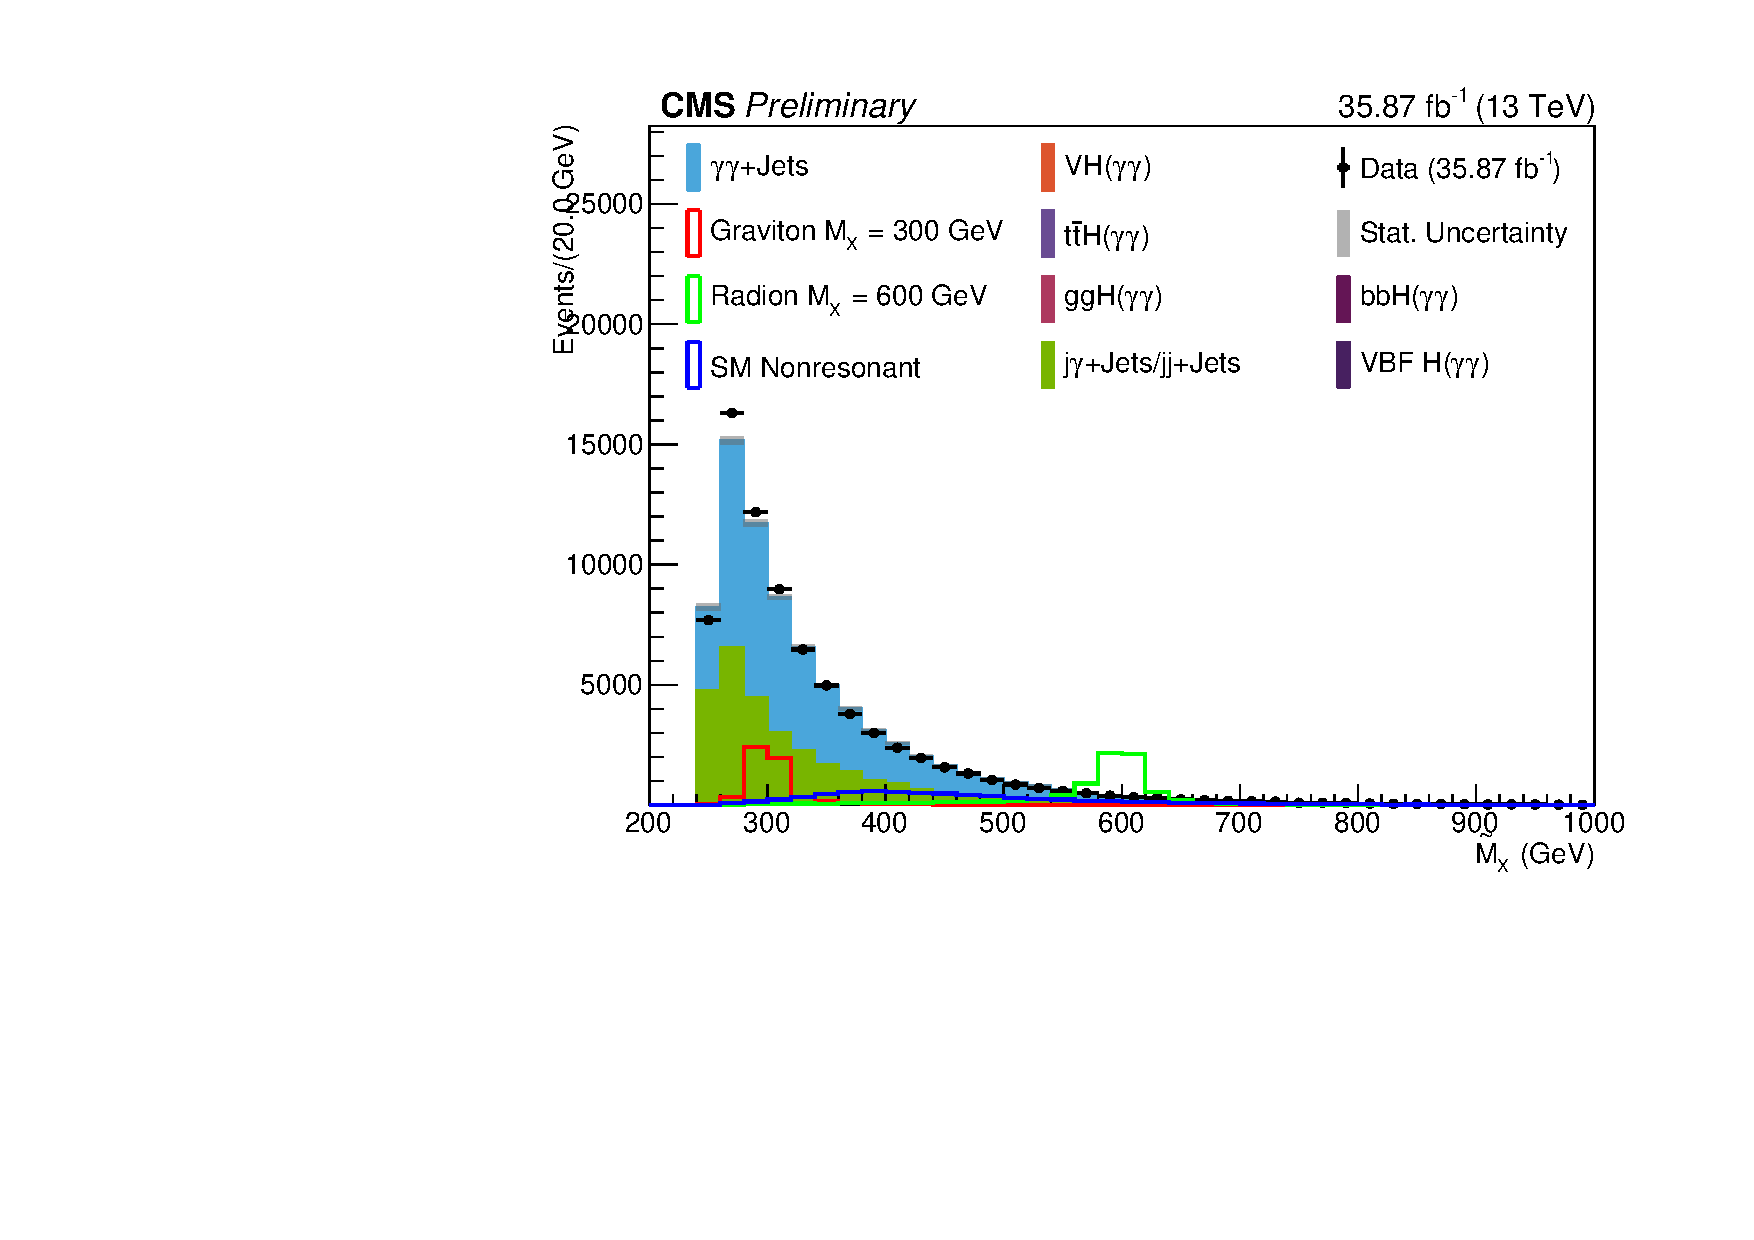
\includegraphics[width=0.45\textwidth]{figures/sec-control/NP_MXprime.pdf}\hfil
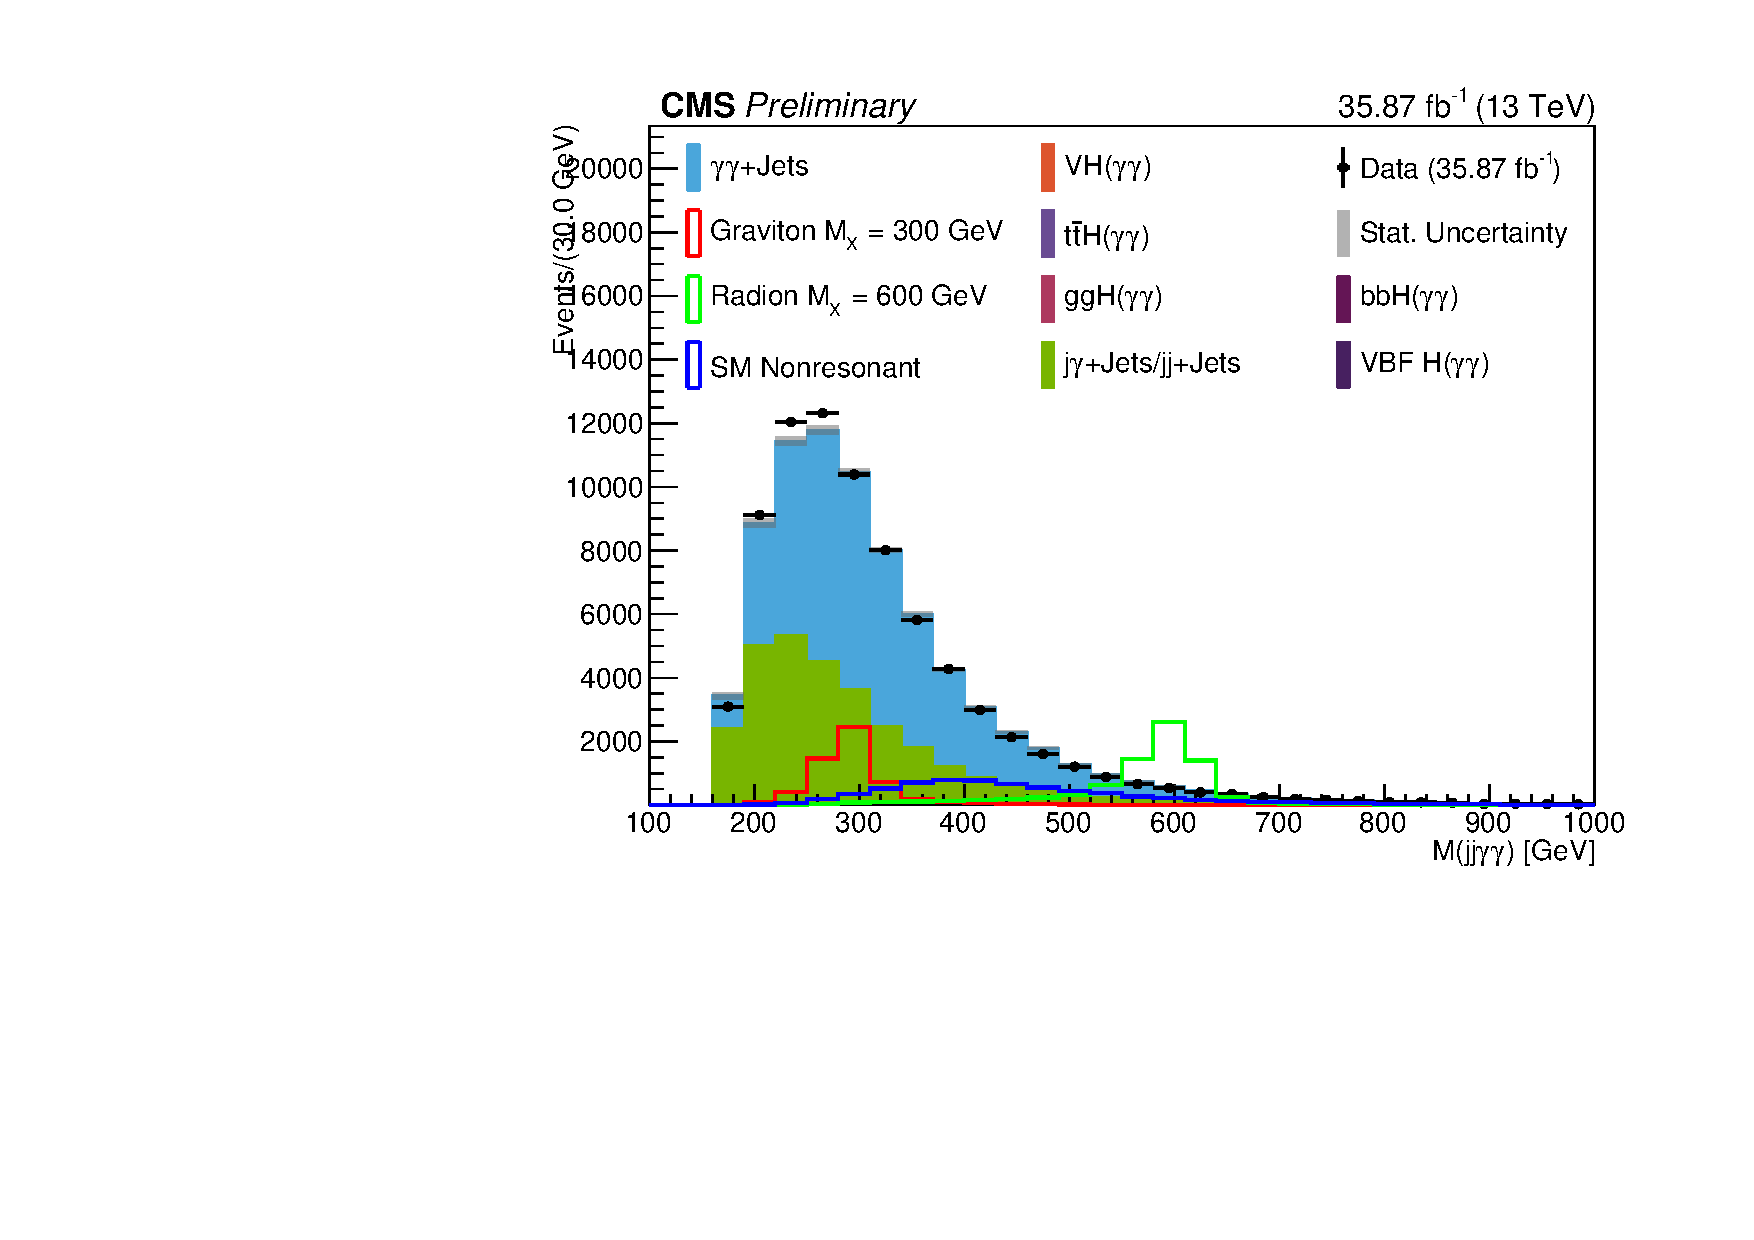
\includegraphics[width=0.45\textwidth]{figures/sec-control/NP_dicandidate_Mass.pdf}\hfil
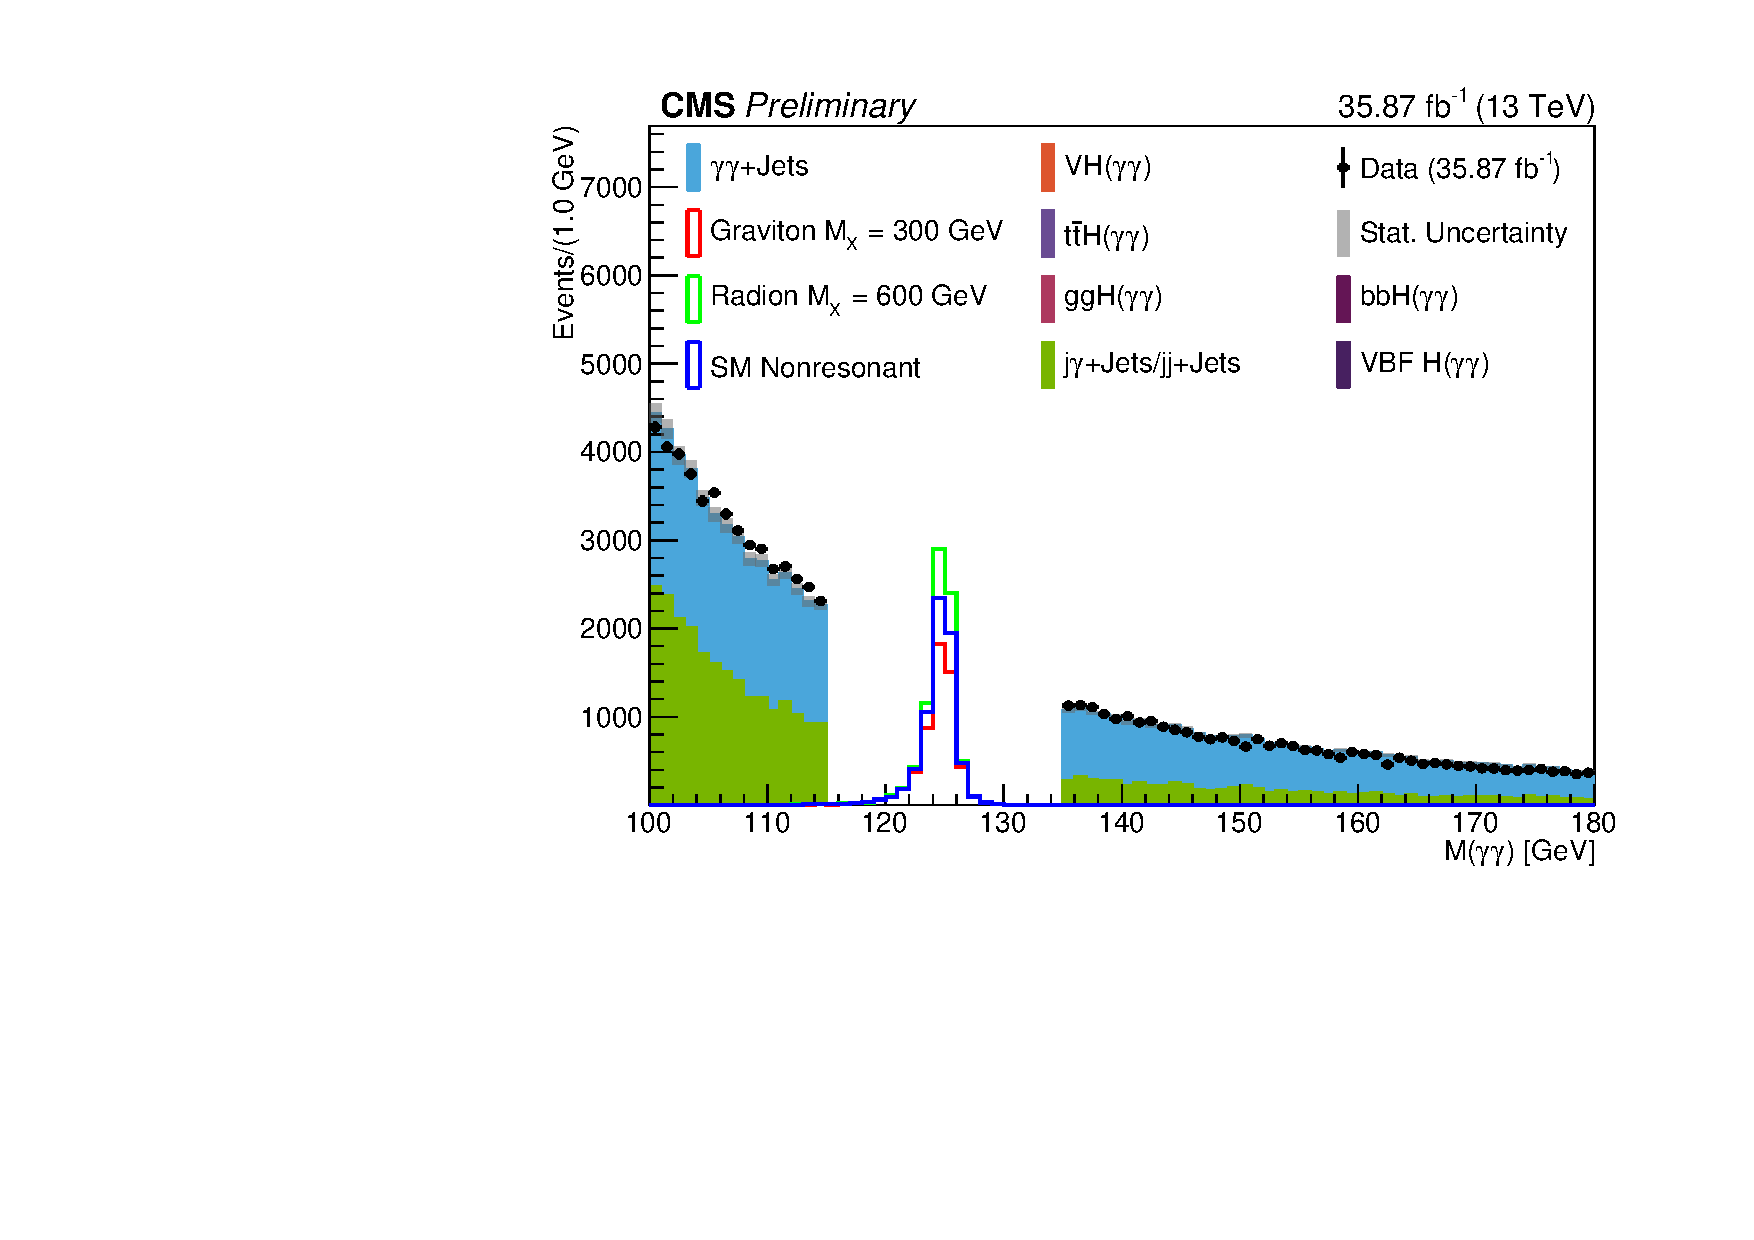
\includegraphics[width=0.45\textwidth]{figures/sec-control/NP_diPho_Mass.pdf}\hfil
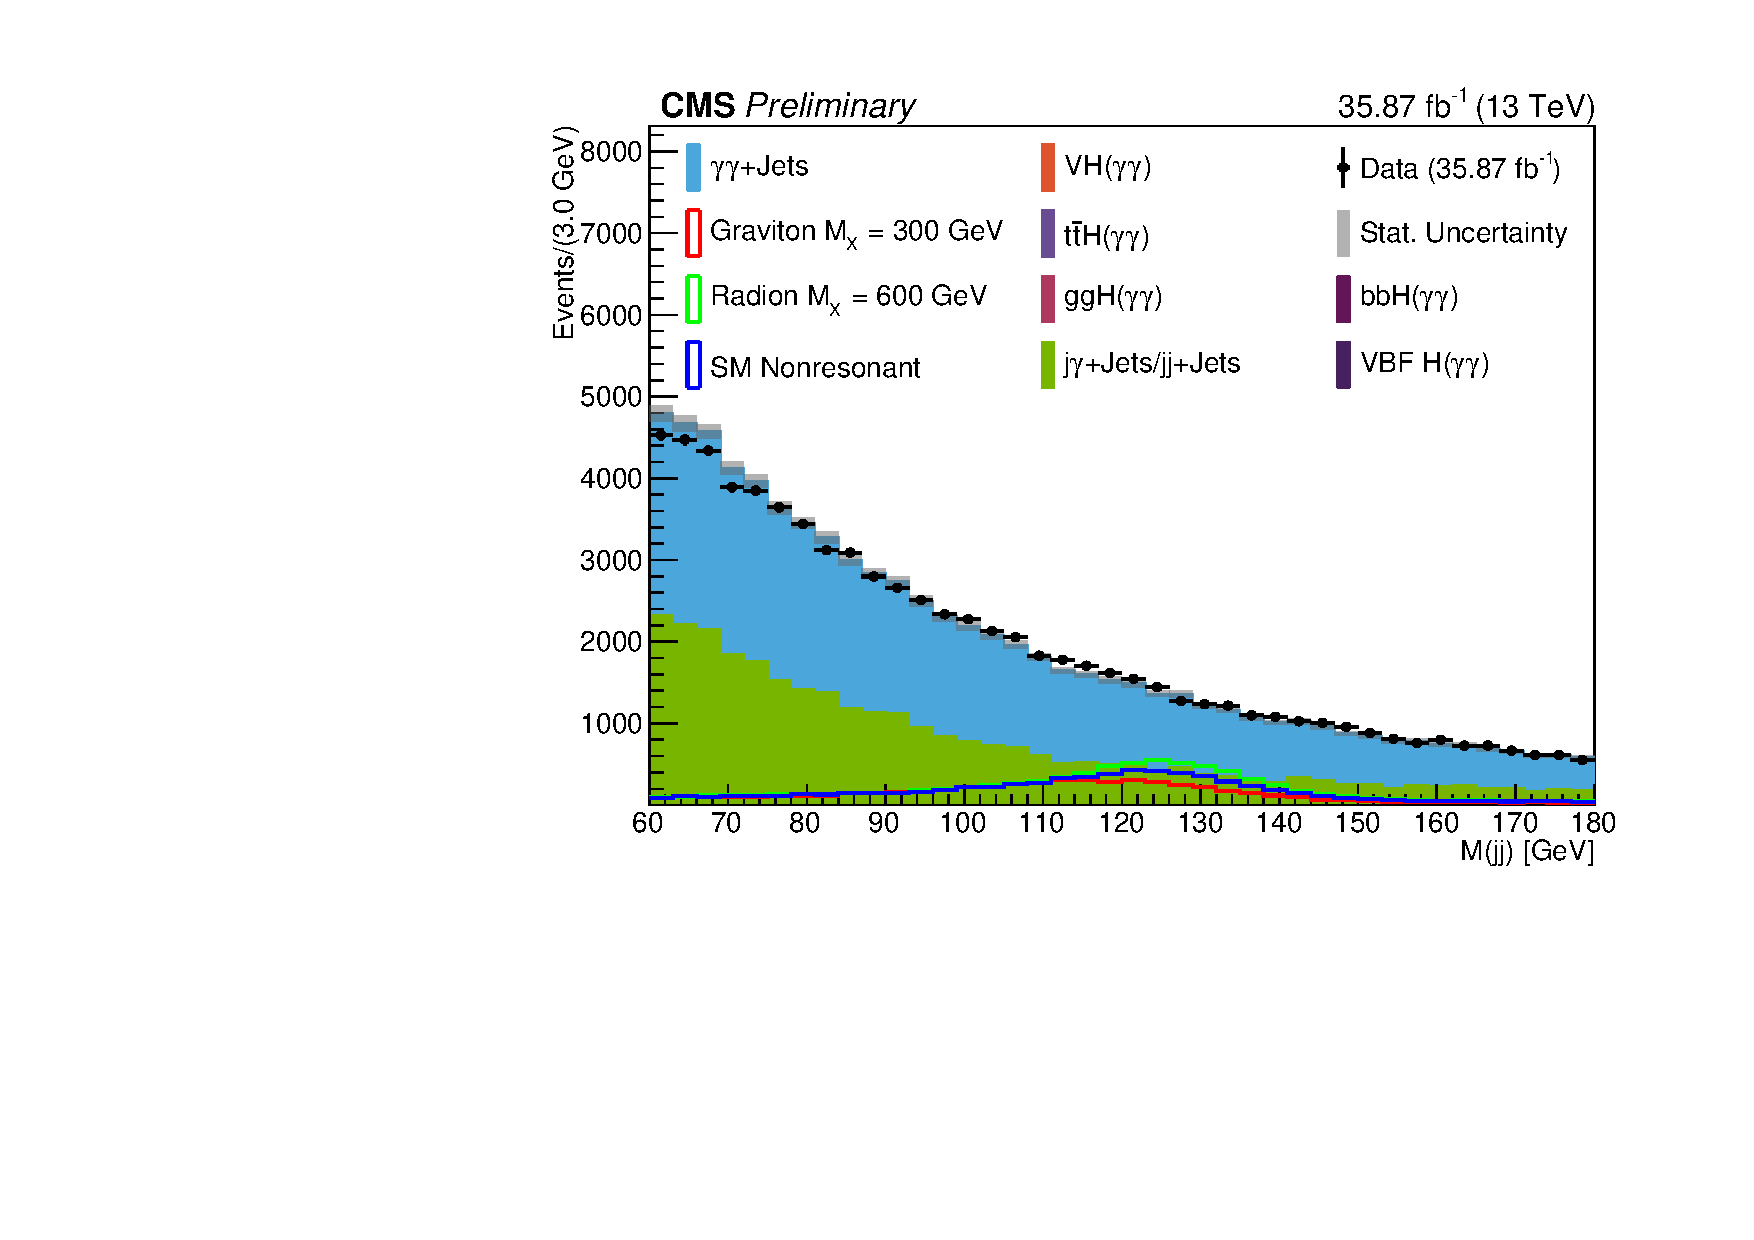
\includegraphics[width=0.45\textwidth]{figures/sec-control/NP_diJet_Mass.pdf}\hfil
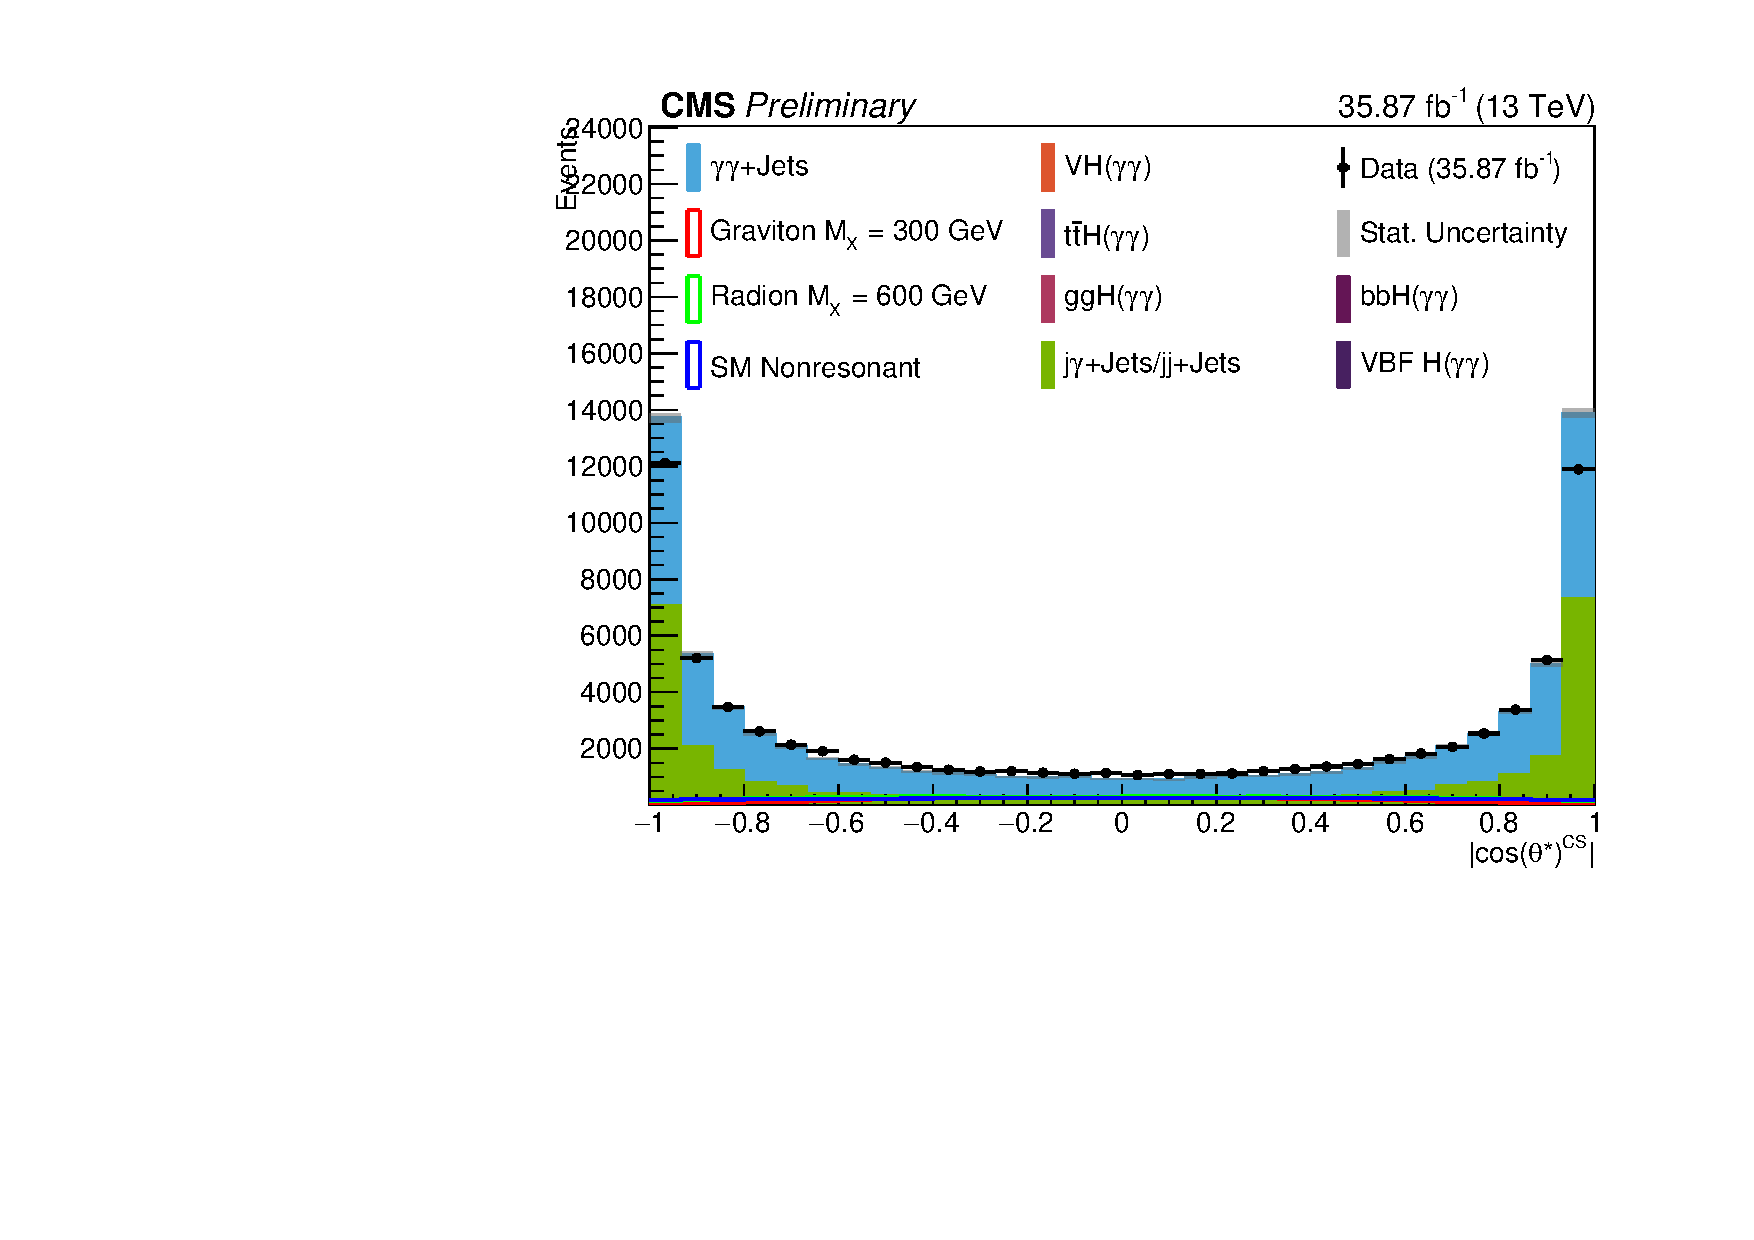
\includegraphics[width=0.45\textwidth]{figures/sec-control/NP_CosThetaStar_CS.pdf}\hfil
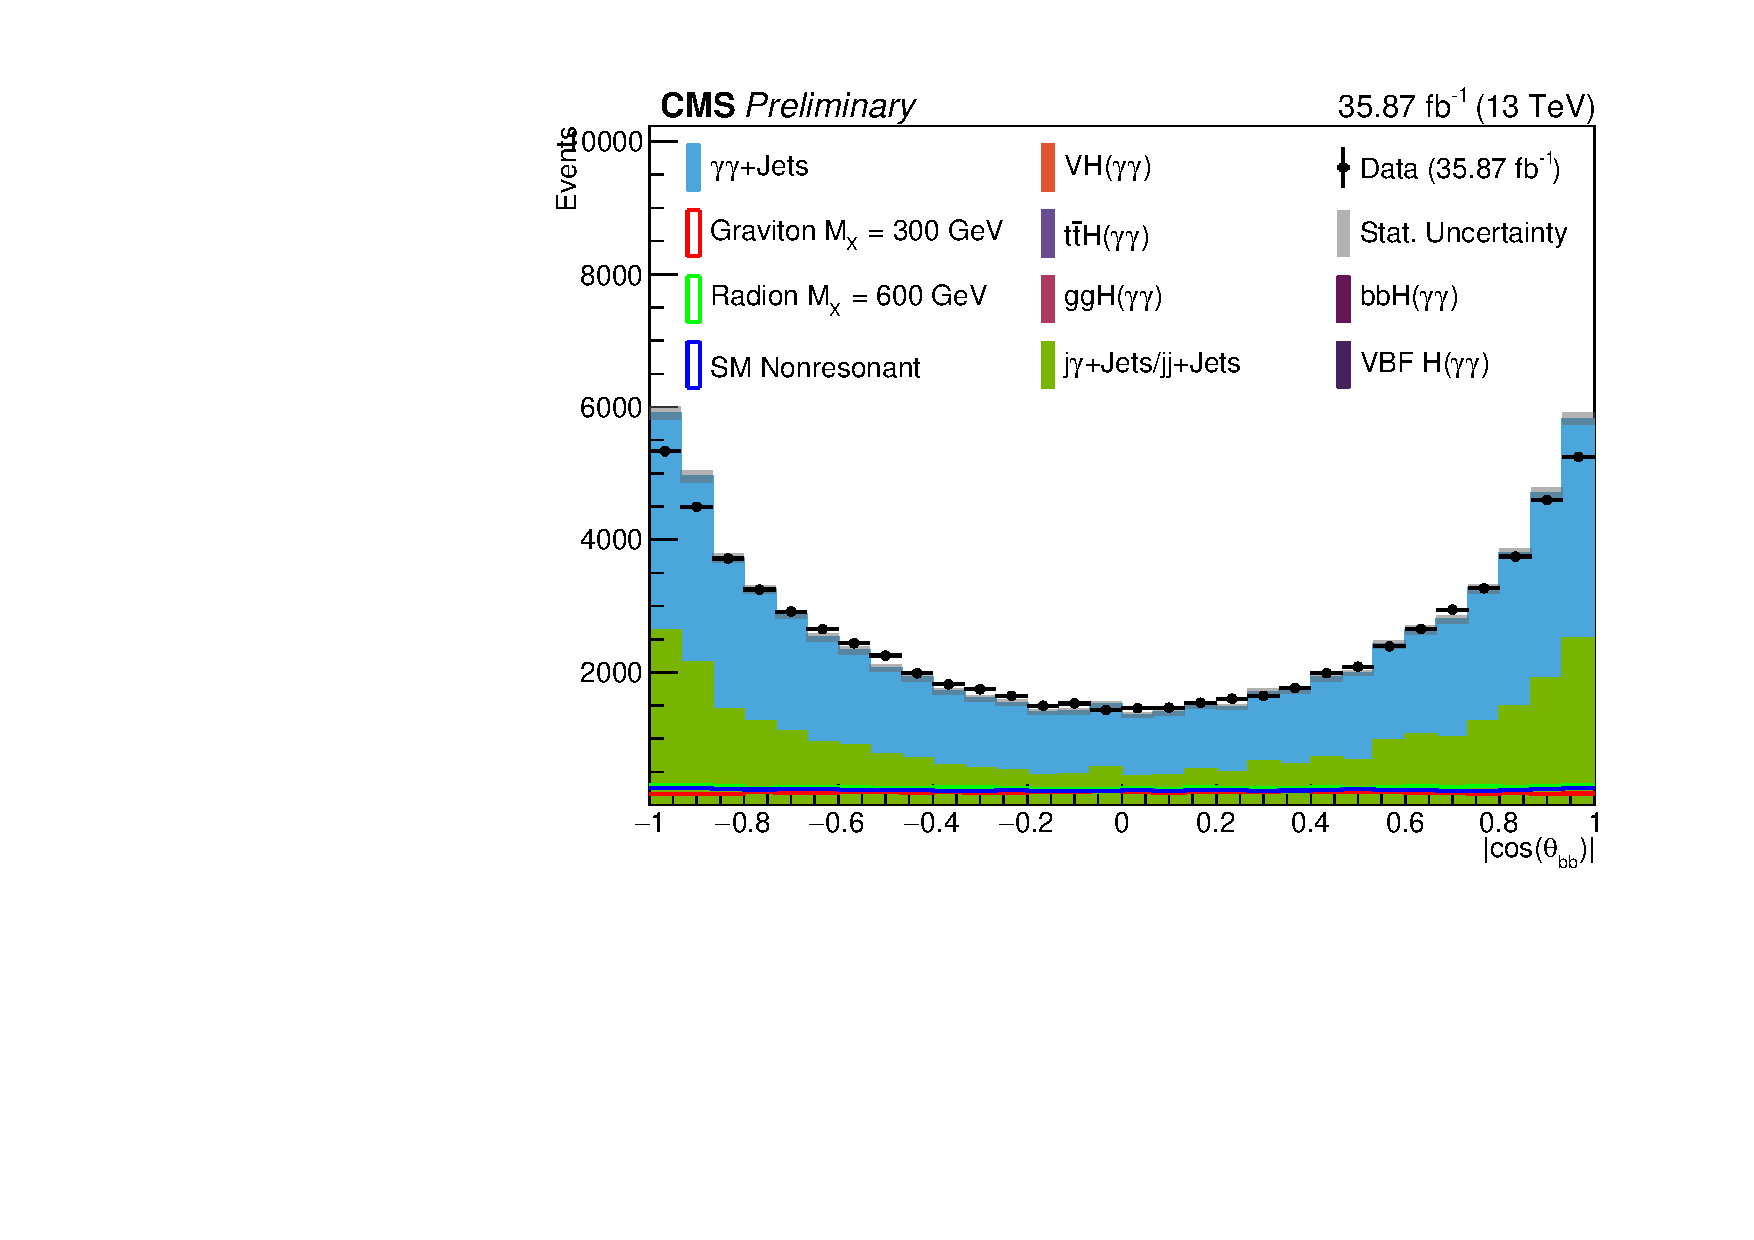
\includegraphics[width=0.45\textwidth]{figures/sec-control/NP_CosTheta_bb.pdf}\hfil

  \caption{Distributions of data and MC for the signal region with the blinding region removed. Top left: $\Mtilde$. Top right: $\Mjjgg$. Center left: $\Mgg$. Center right: $\Mjj$. Bottom left: $|cos(\theta^{*}_{CS})|$. Bottom right: $|cos(\theta^{*}_{bb})|$.}
\label{fig:cp_mgg1}
\end{figure*}

%\begin{figure*}[thb]
%  \centering
%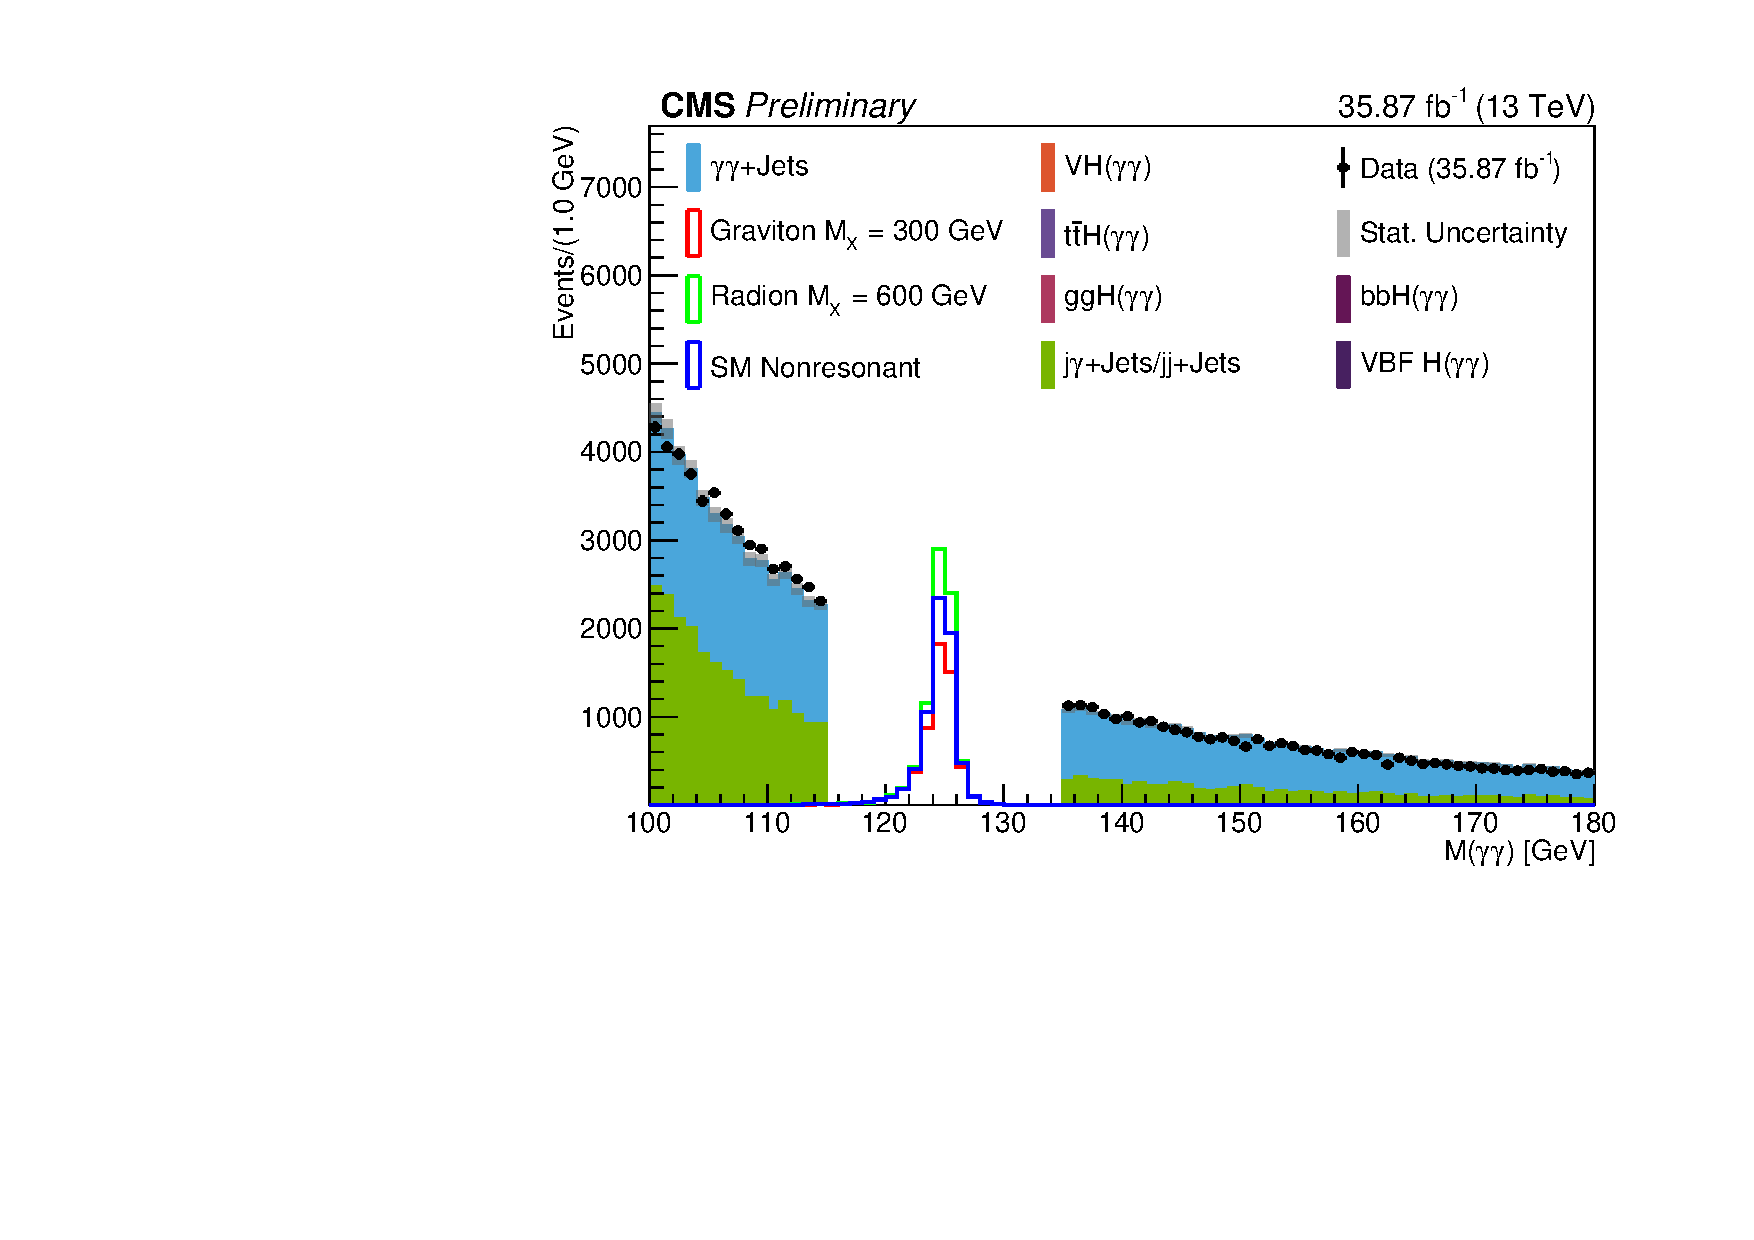
\includegraphics[width=0.45\textwidth]{figures/sec-control/NP_diPho_Mass.pdf}\hfil
%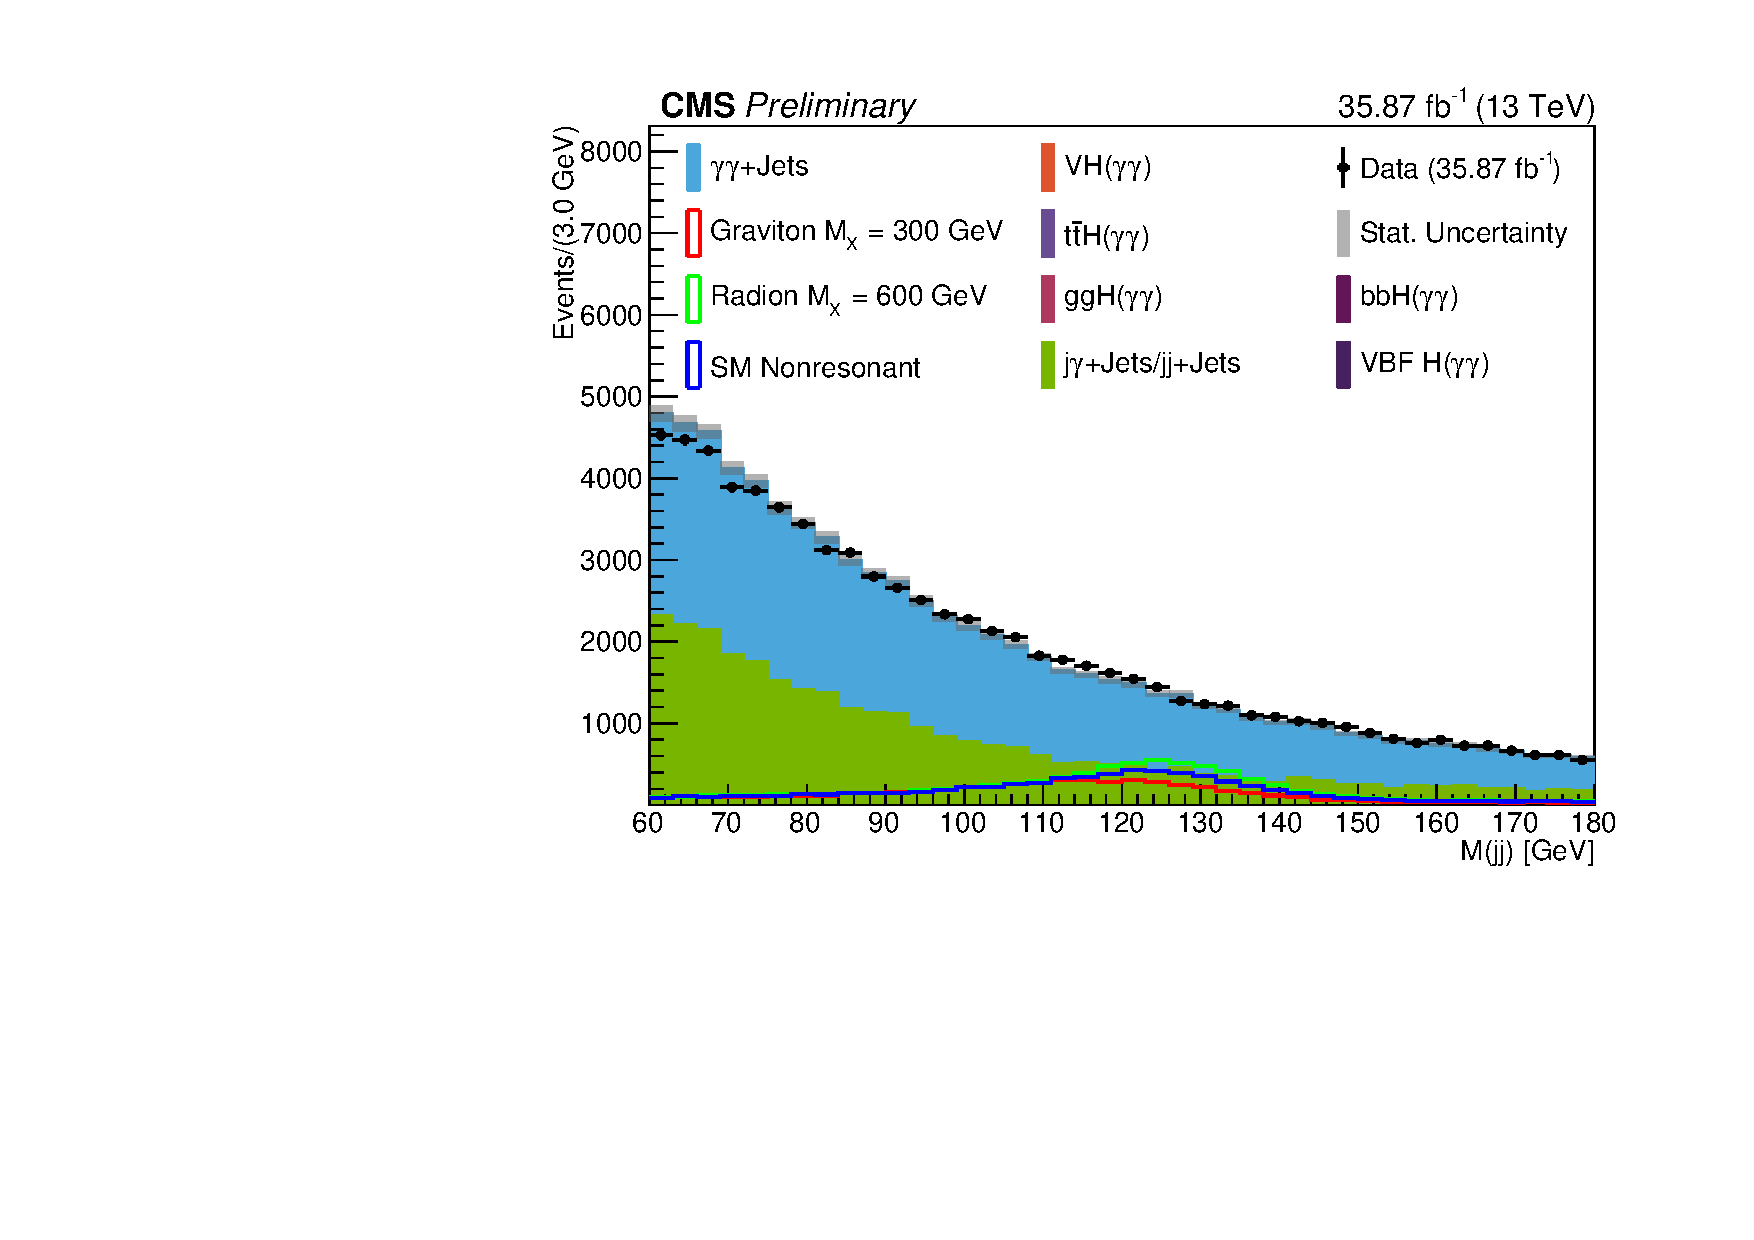
\includegraphics[width=0.45\textwidth]{figures/sec-control/NP_diJet_Mass.pdf}\hfil
%  \caption{Distributions of data and MC for the signal region with the blinding region removed.}
%\label{fig:cp_mgg2}
%\end{figure*}
%\begin{figure*}[thb]
%  \centering
%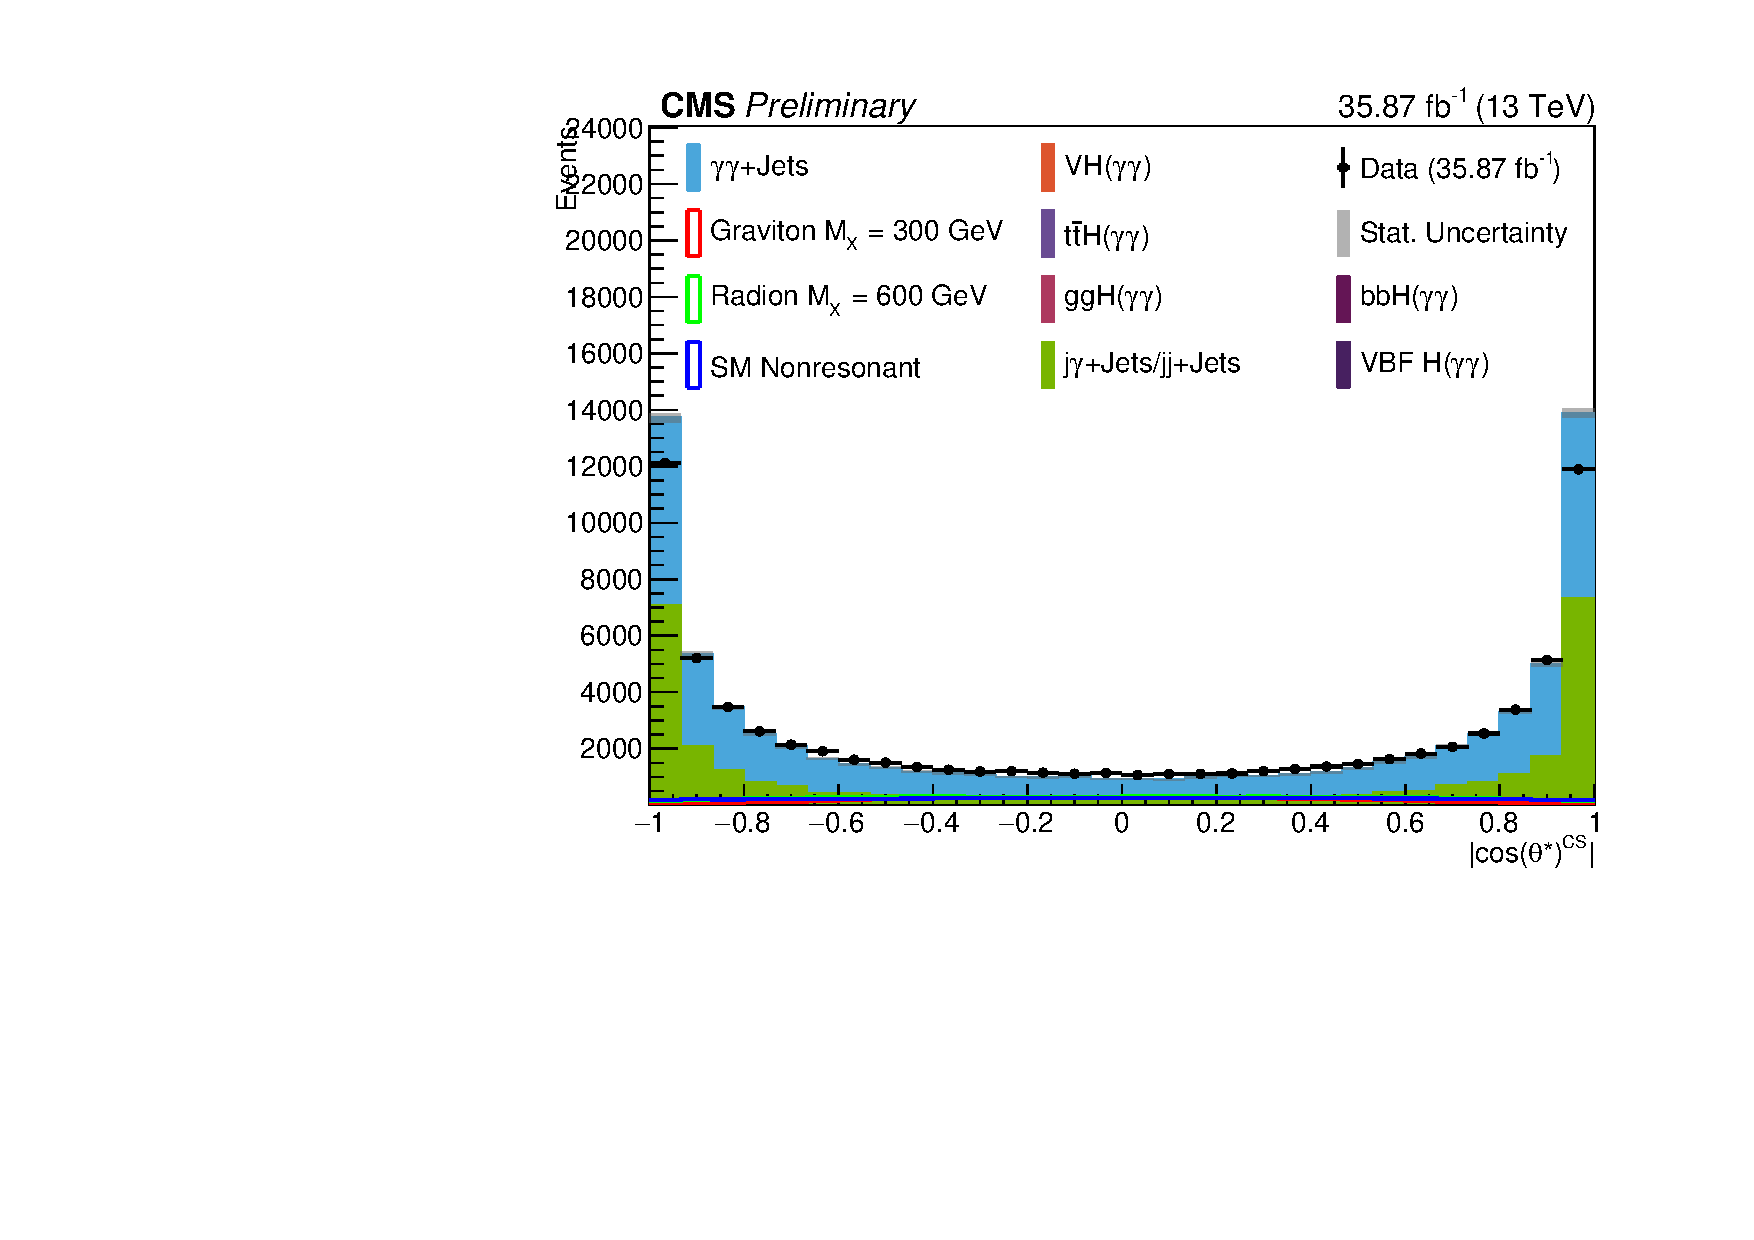
\includegraphics[width=0.45\textwidth]{figures/sec-control/NP_CosThetaStar_CS.pdf}\hfil
%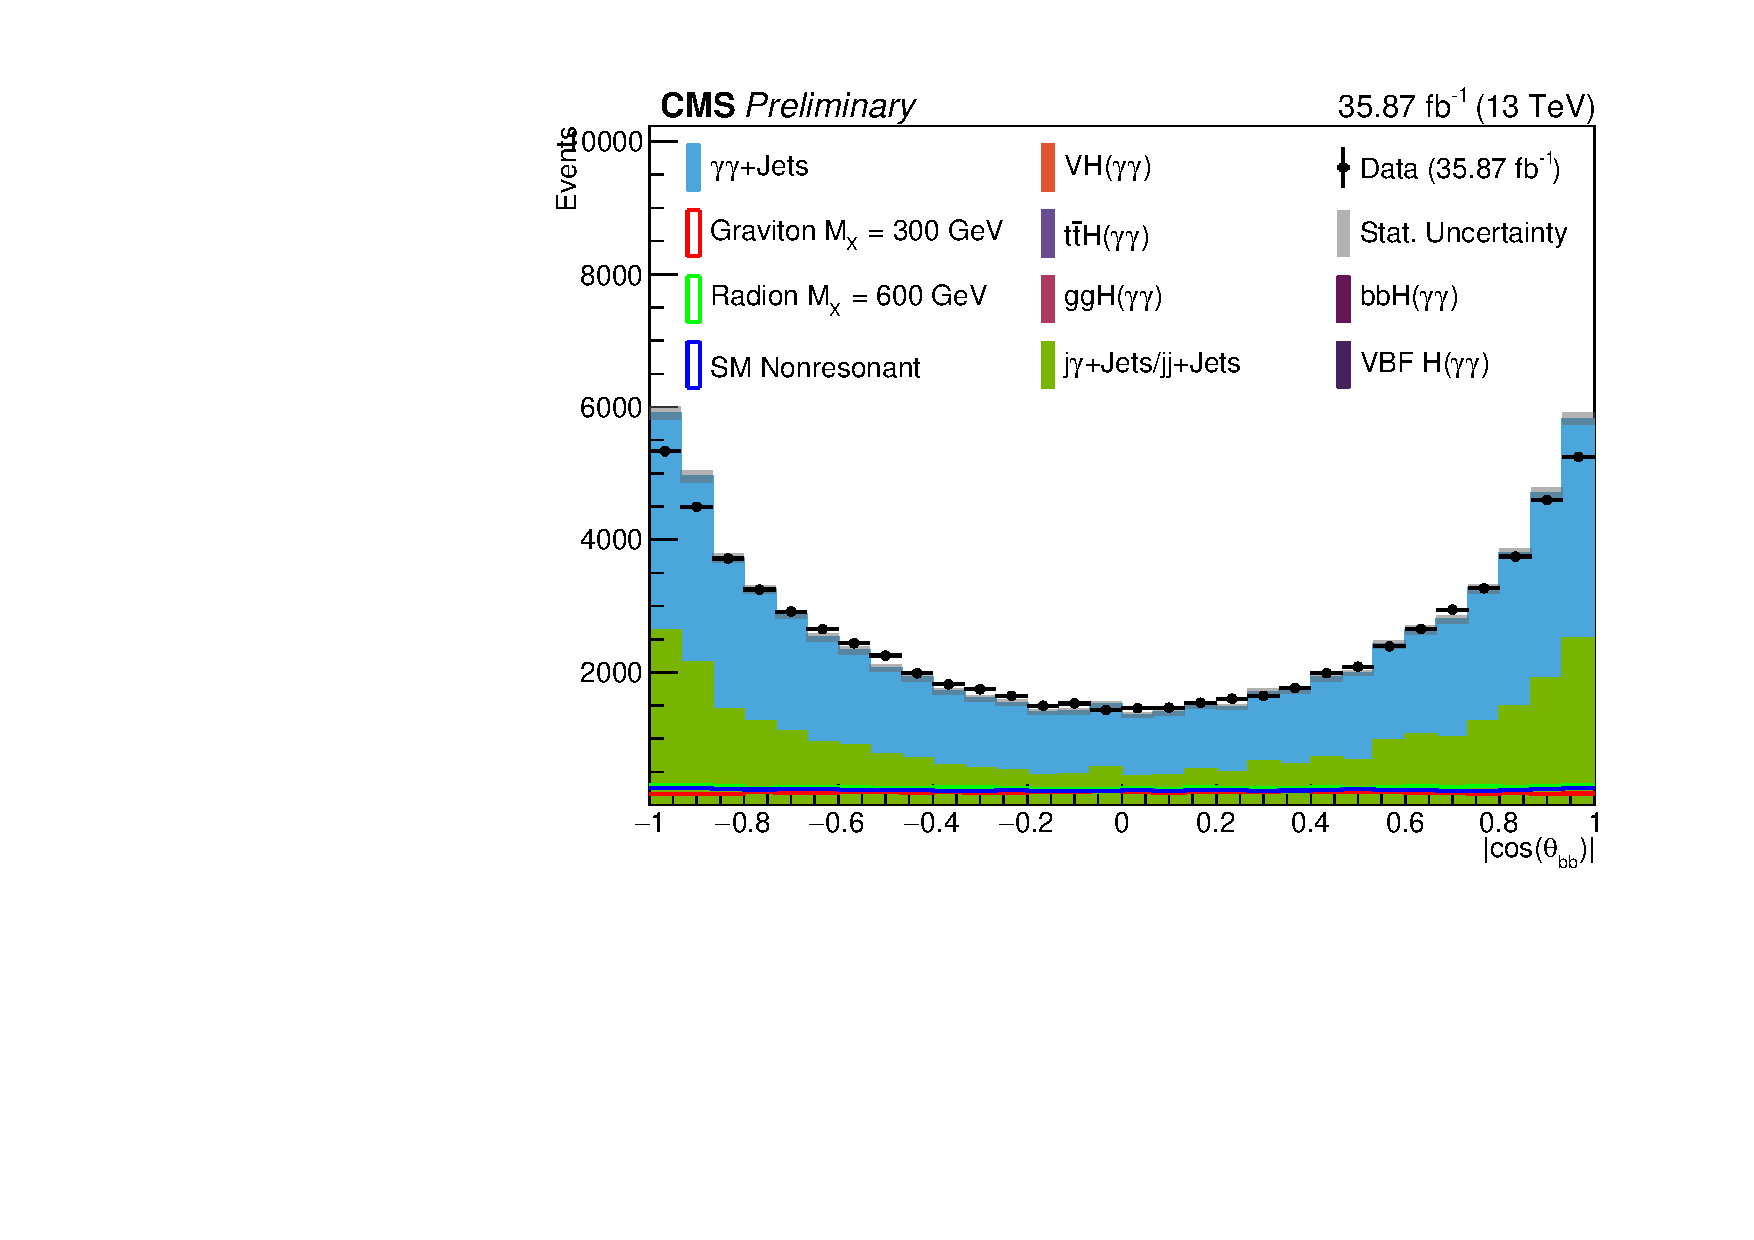
\includegraphics[width=0.45\textwidth]{figures/sec-control/NP_CosTheta_bb.pdf}\hfil
%  \caption{Distributions of data and MC for the signal region with the blinding region removed.}
%\label{fig:cp_mgg3}
%\end{figure*}

\begin{figure*}[thb]
  \centering
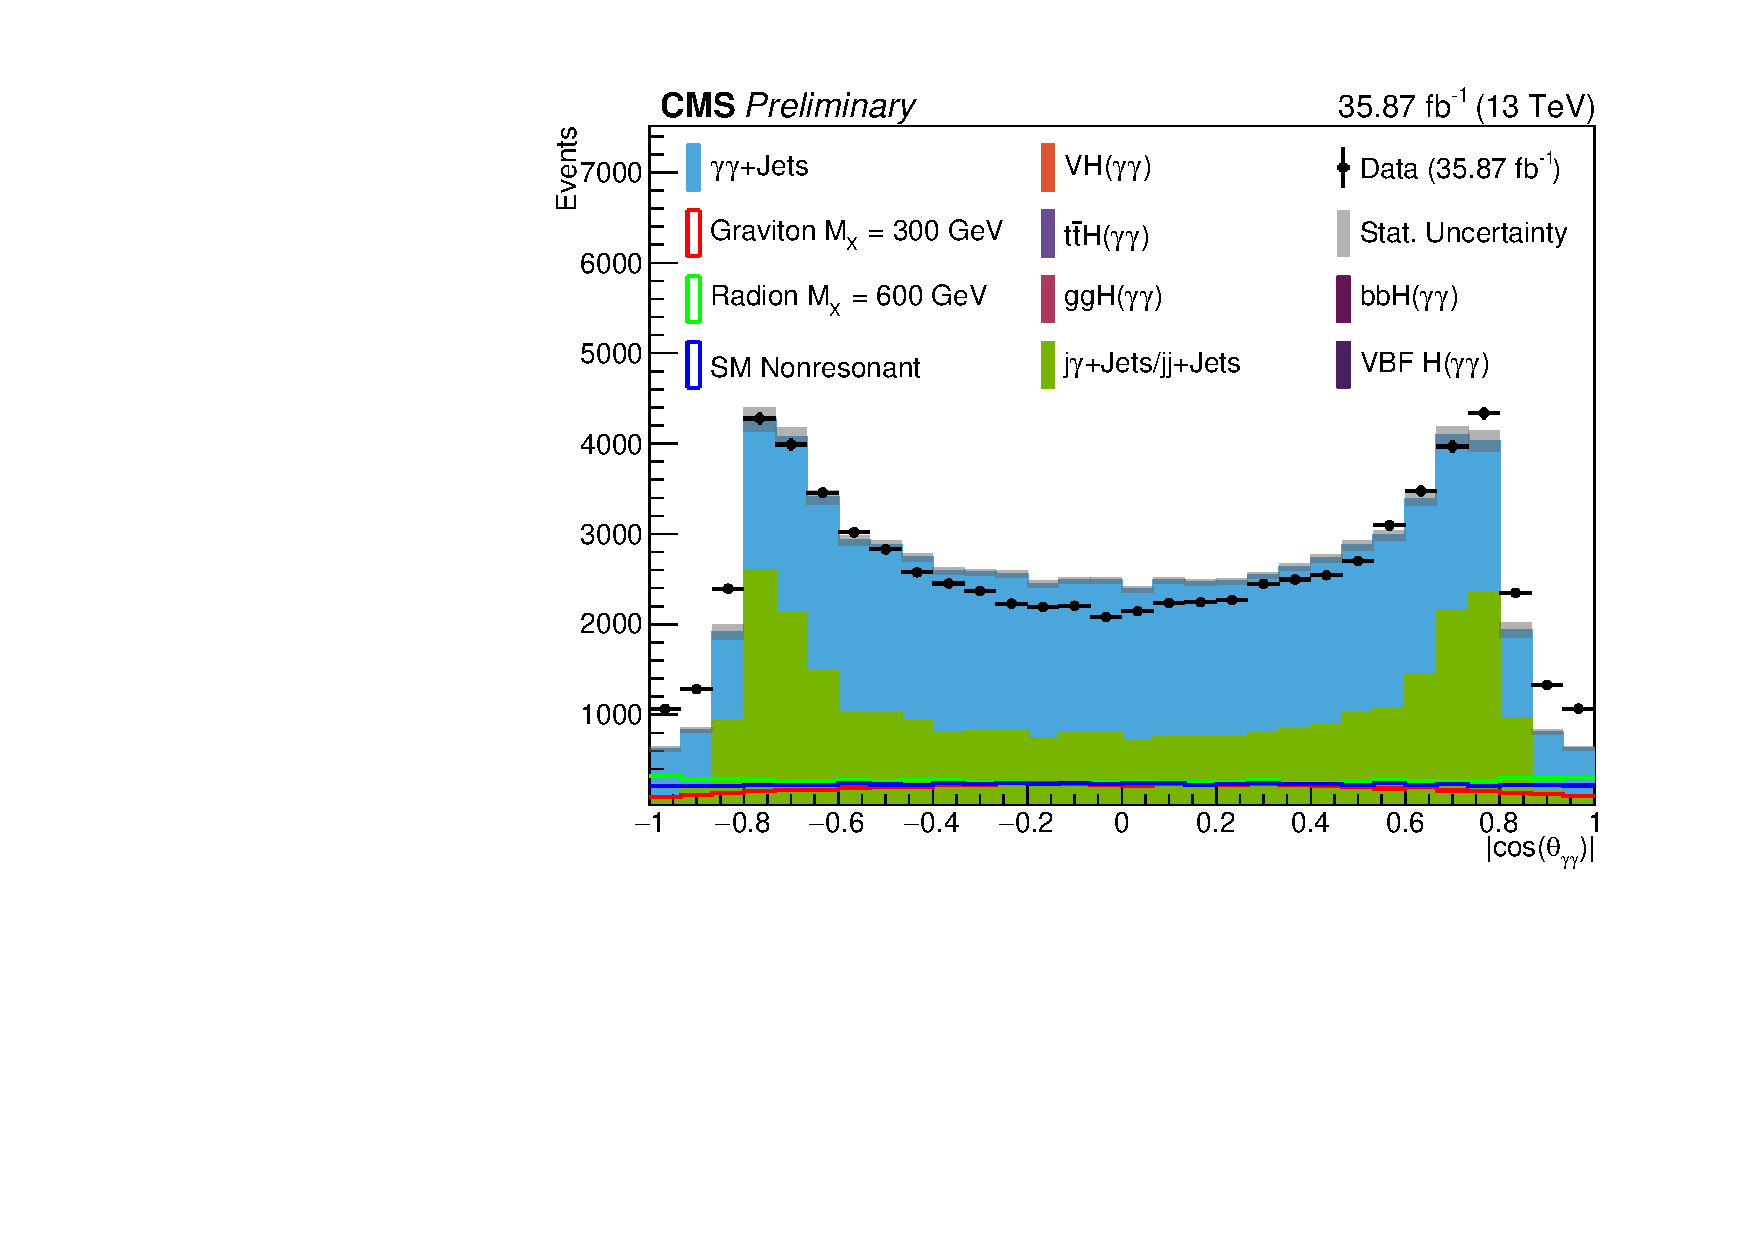
\includegraphics[width=0.45\textwidth]{figures/sec-control/NP_CosTheta_gg.pdf}\hfil
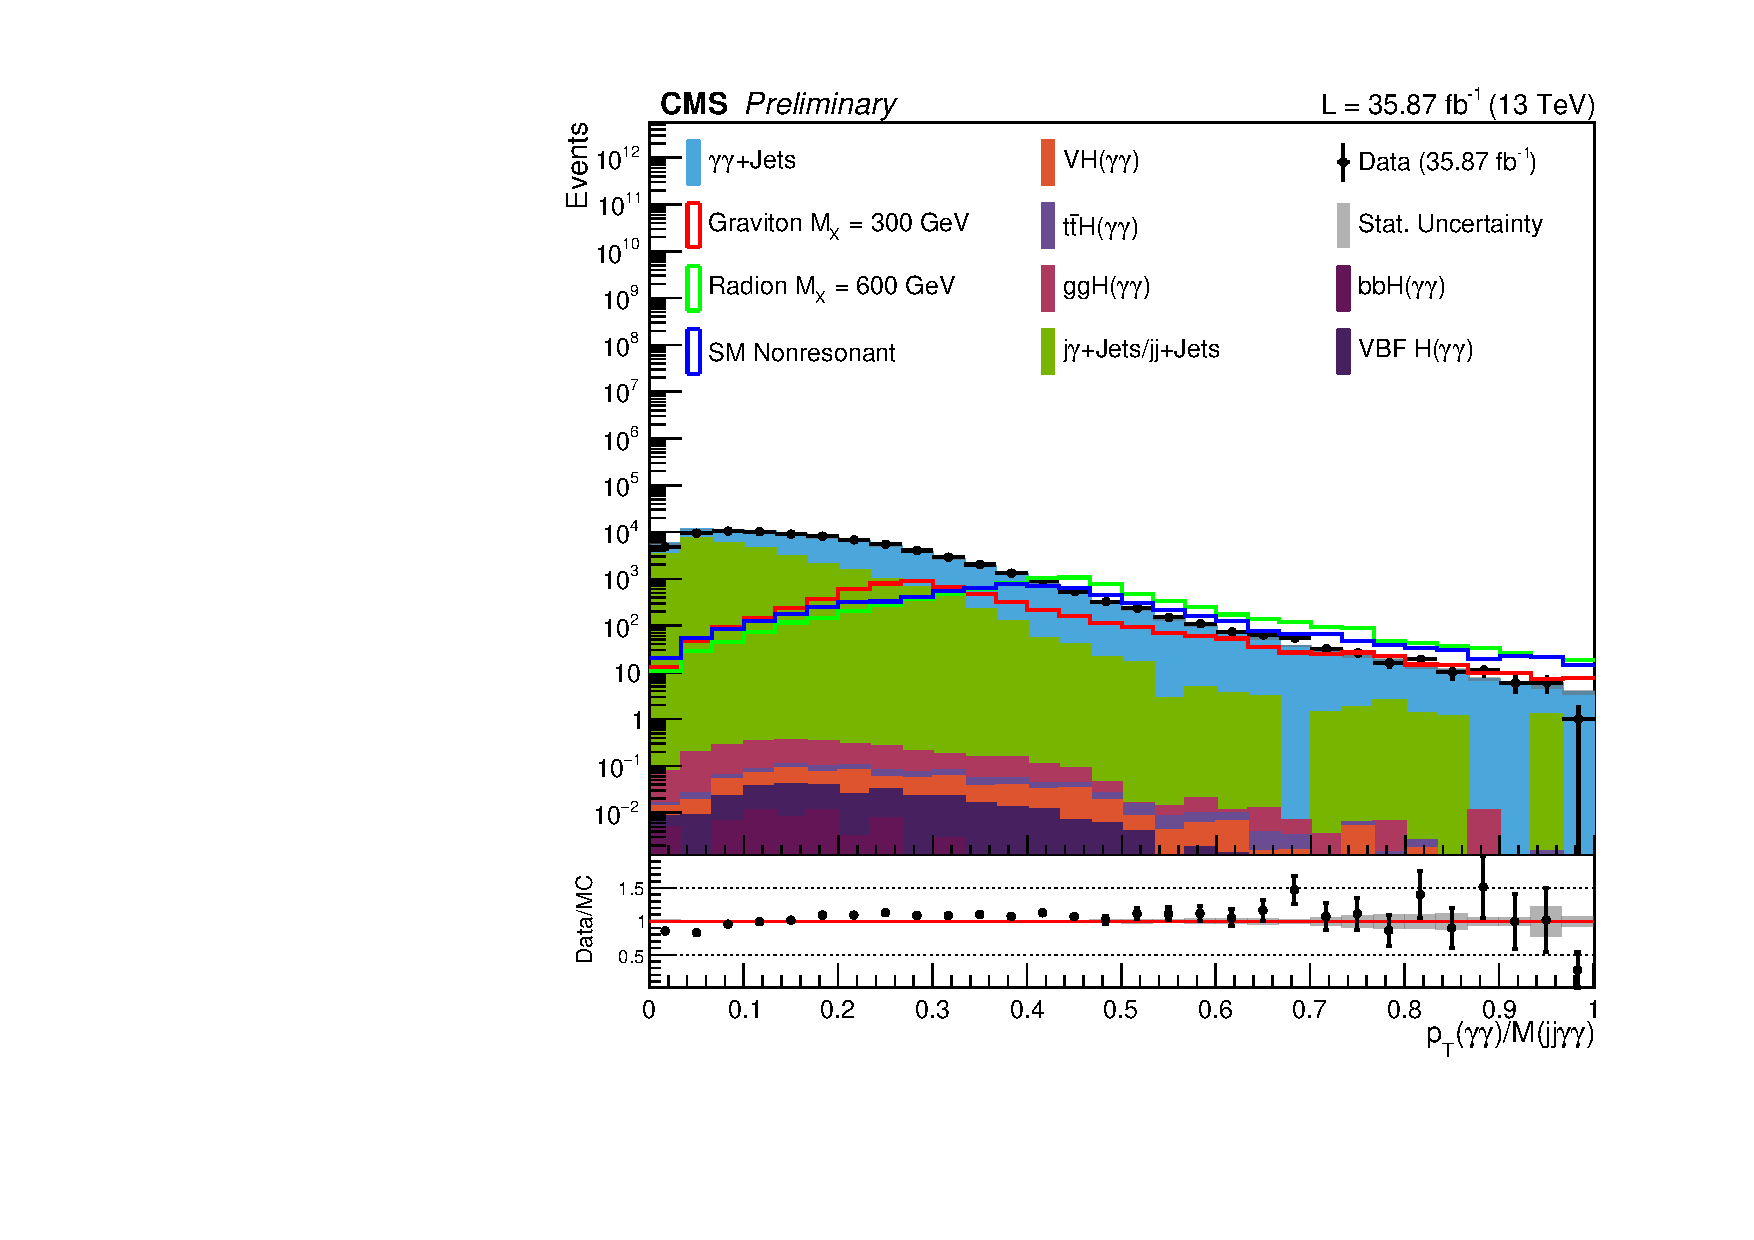
\includegraphics[width=0.45\textwidth]{figures/sec-control/LOG_ggptmjjgg.pdf}\hfil
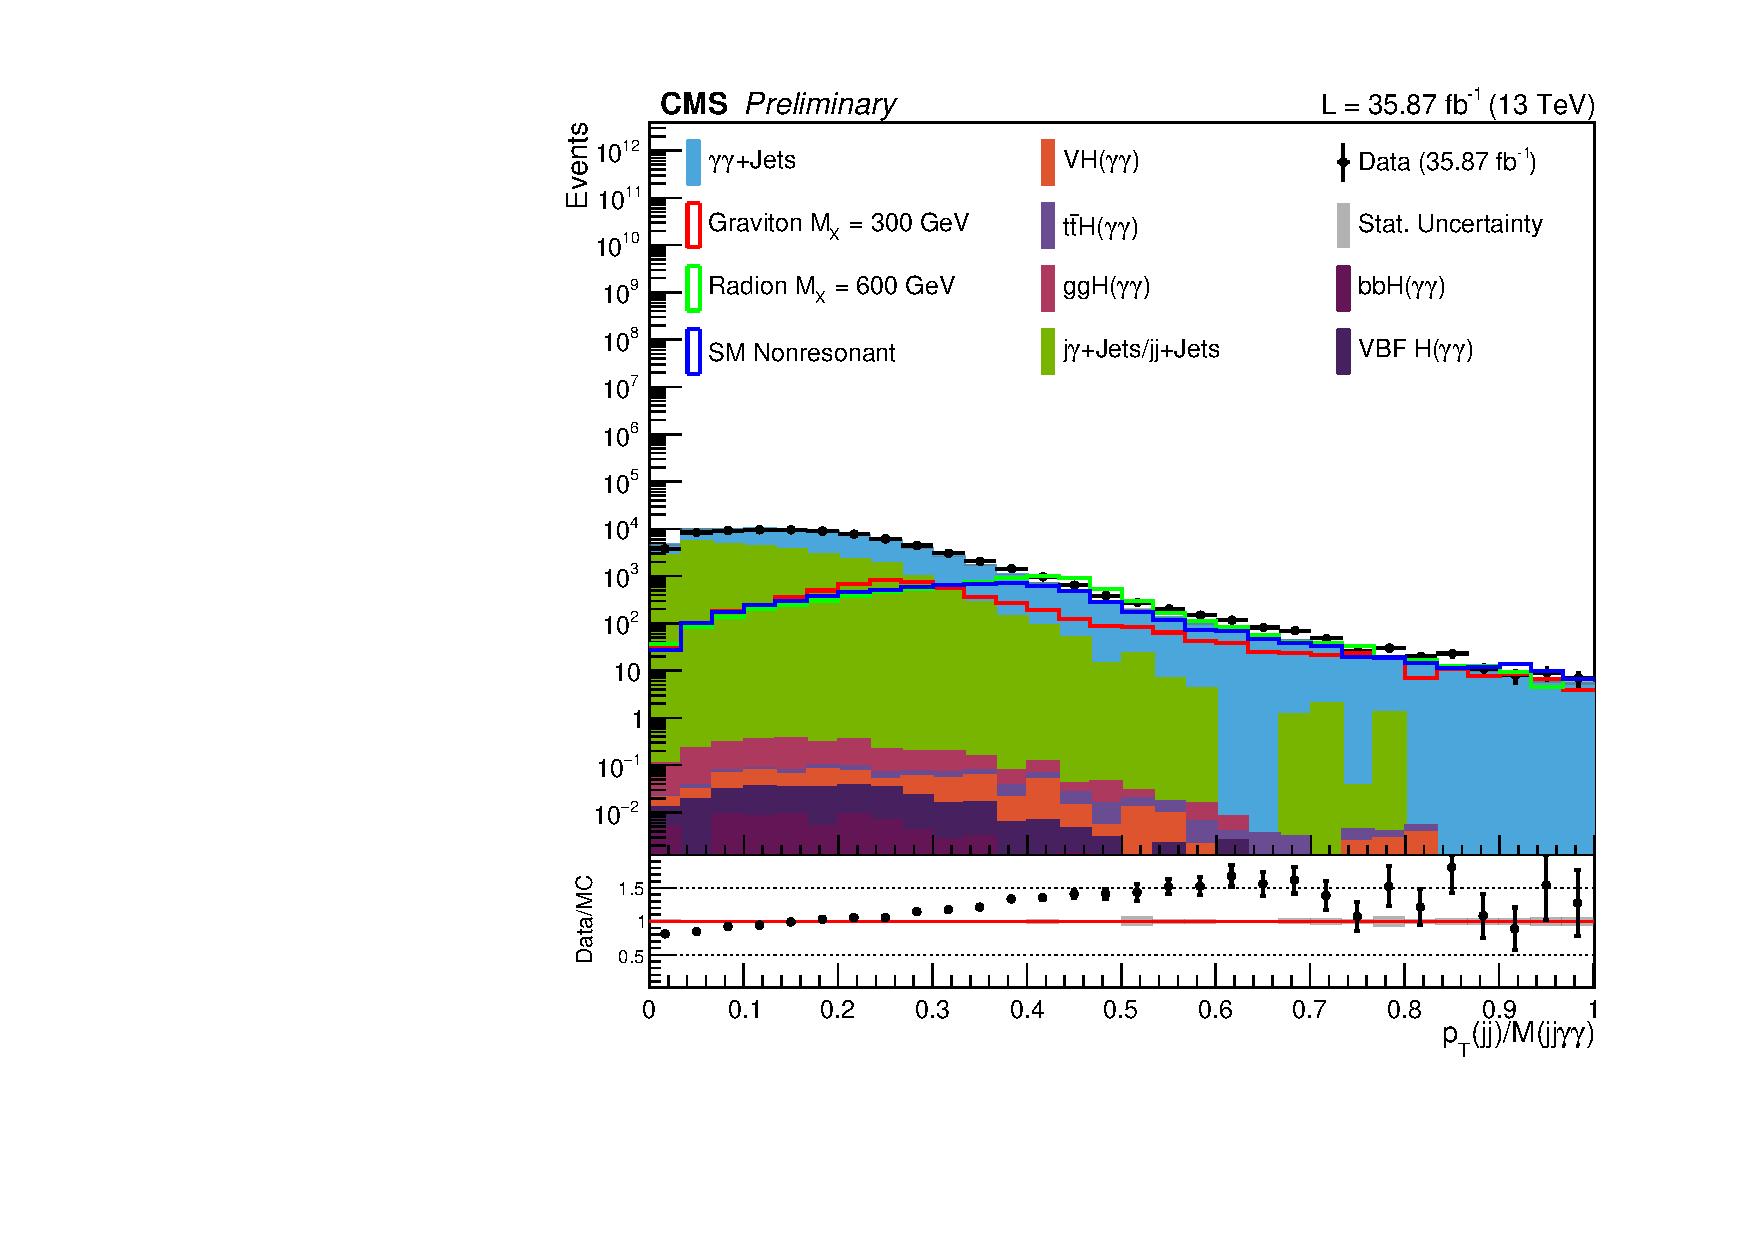
\includegraphics[width=0.45\textwidth]{figures/sec-control/LOG_jjptmjjgg.pdf}\hfil
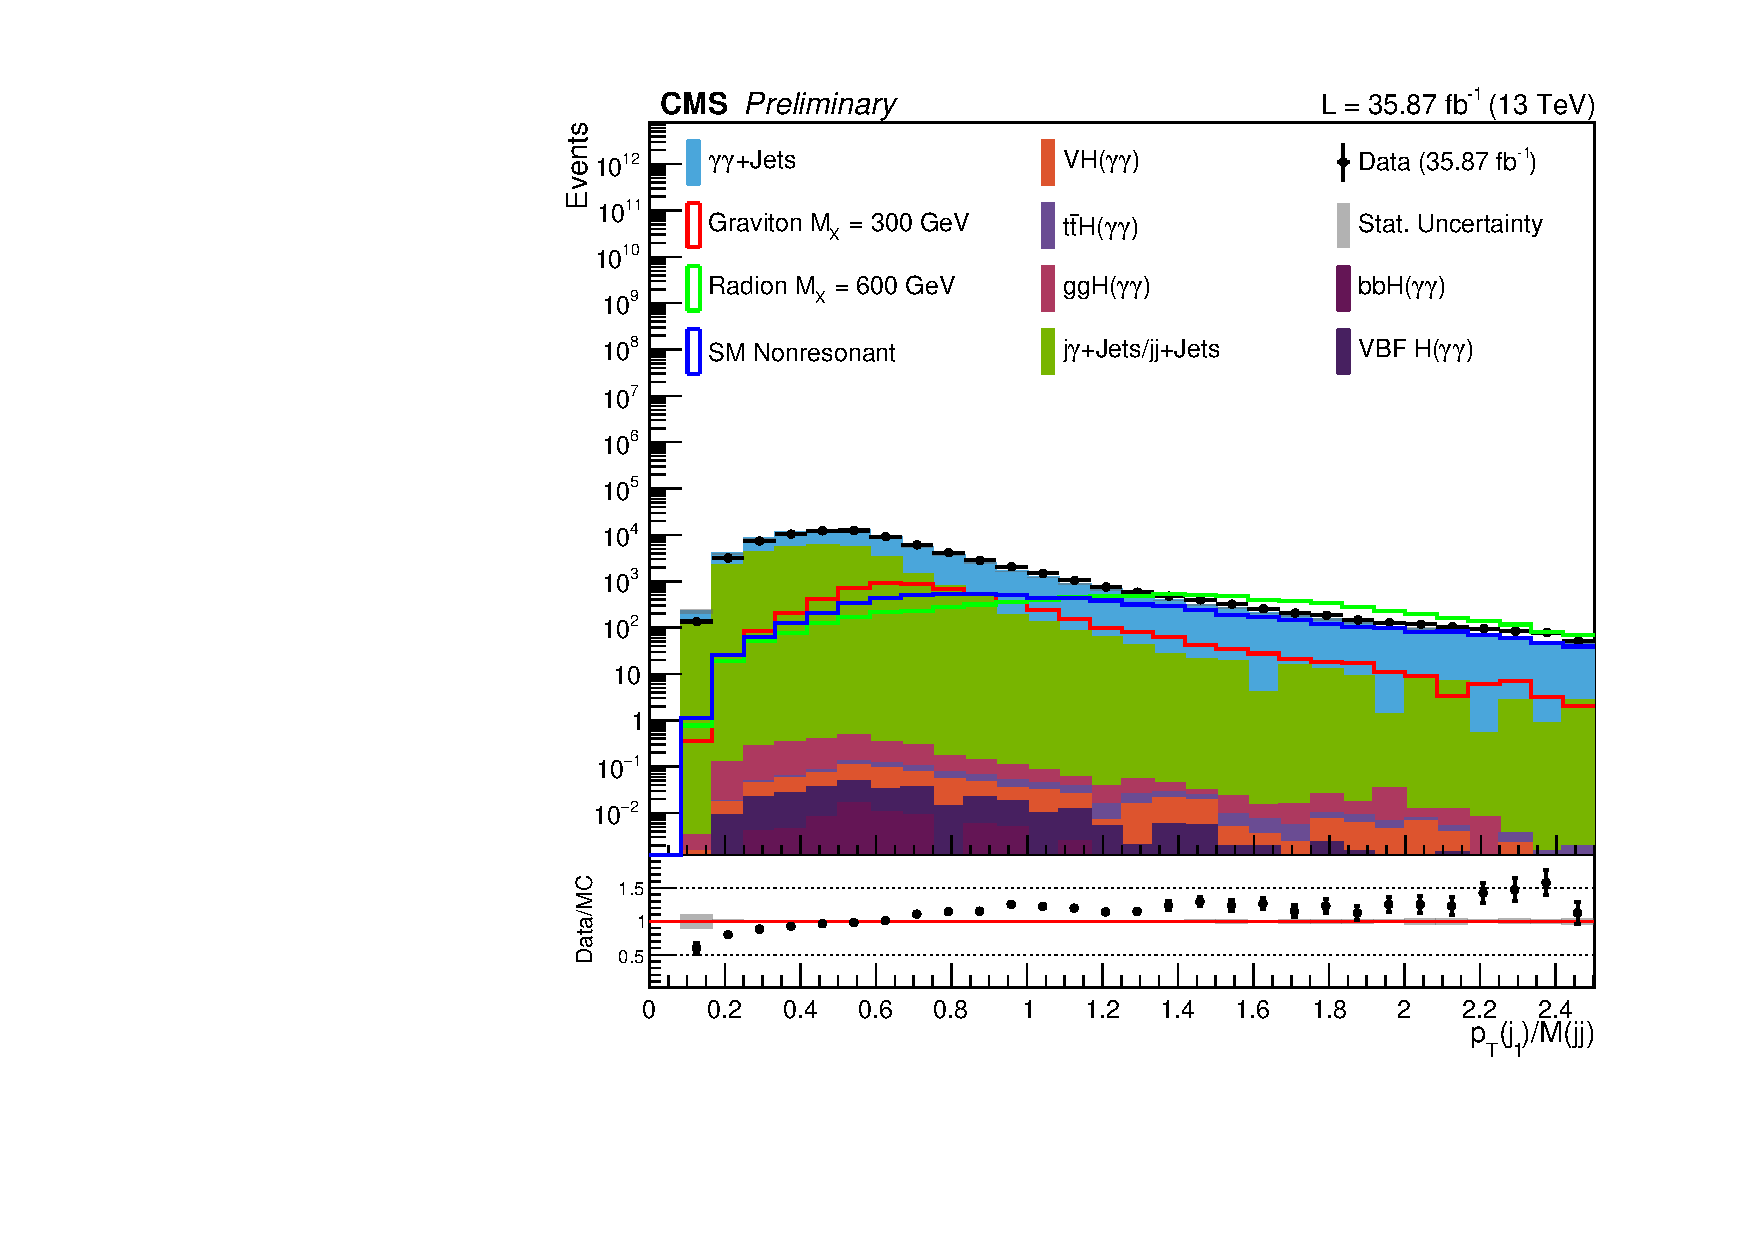
\includegraphics[width=0.45\textwidth]{figures/sec-control/LOG_ljetptmgg}\hfil
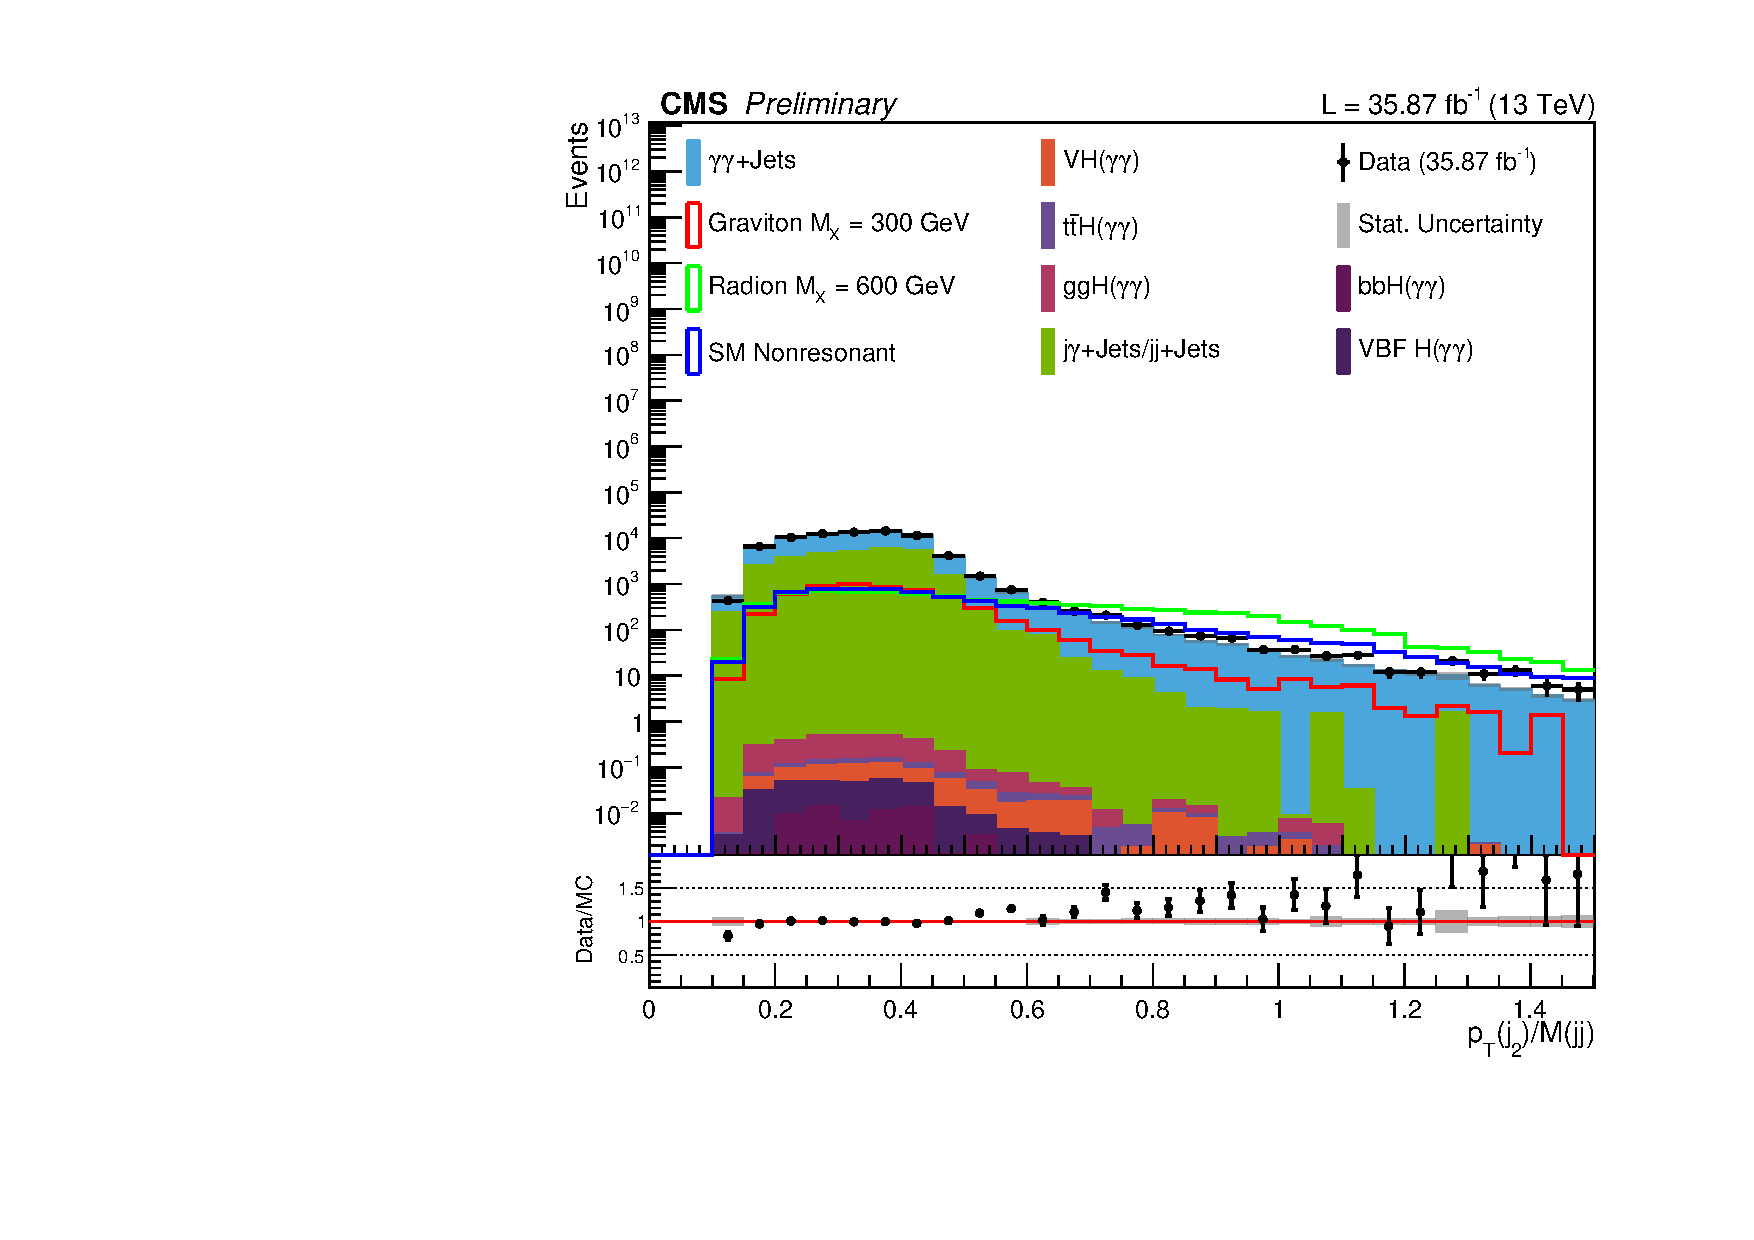
\includegraphics[width=0.45\textwidth]{figures/sec-control/LOG_sjetptmgg}\hfil
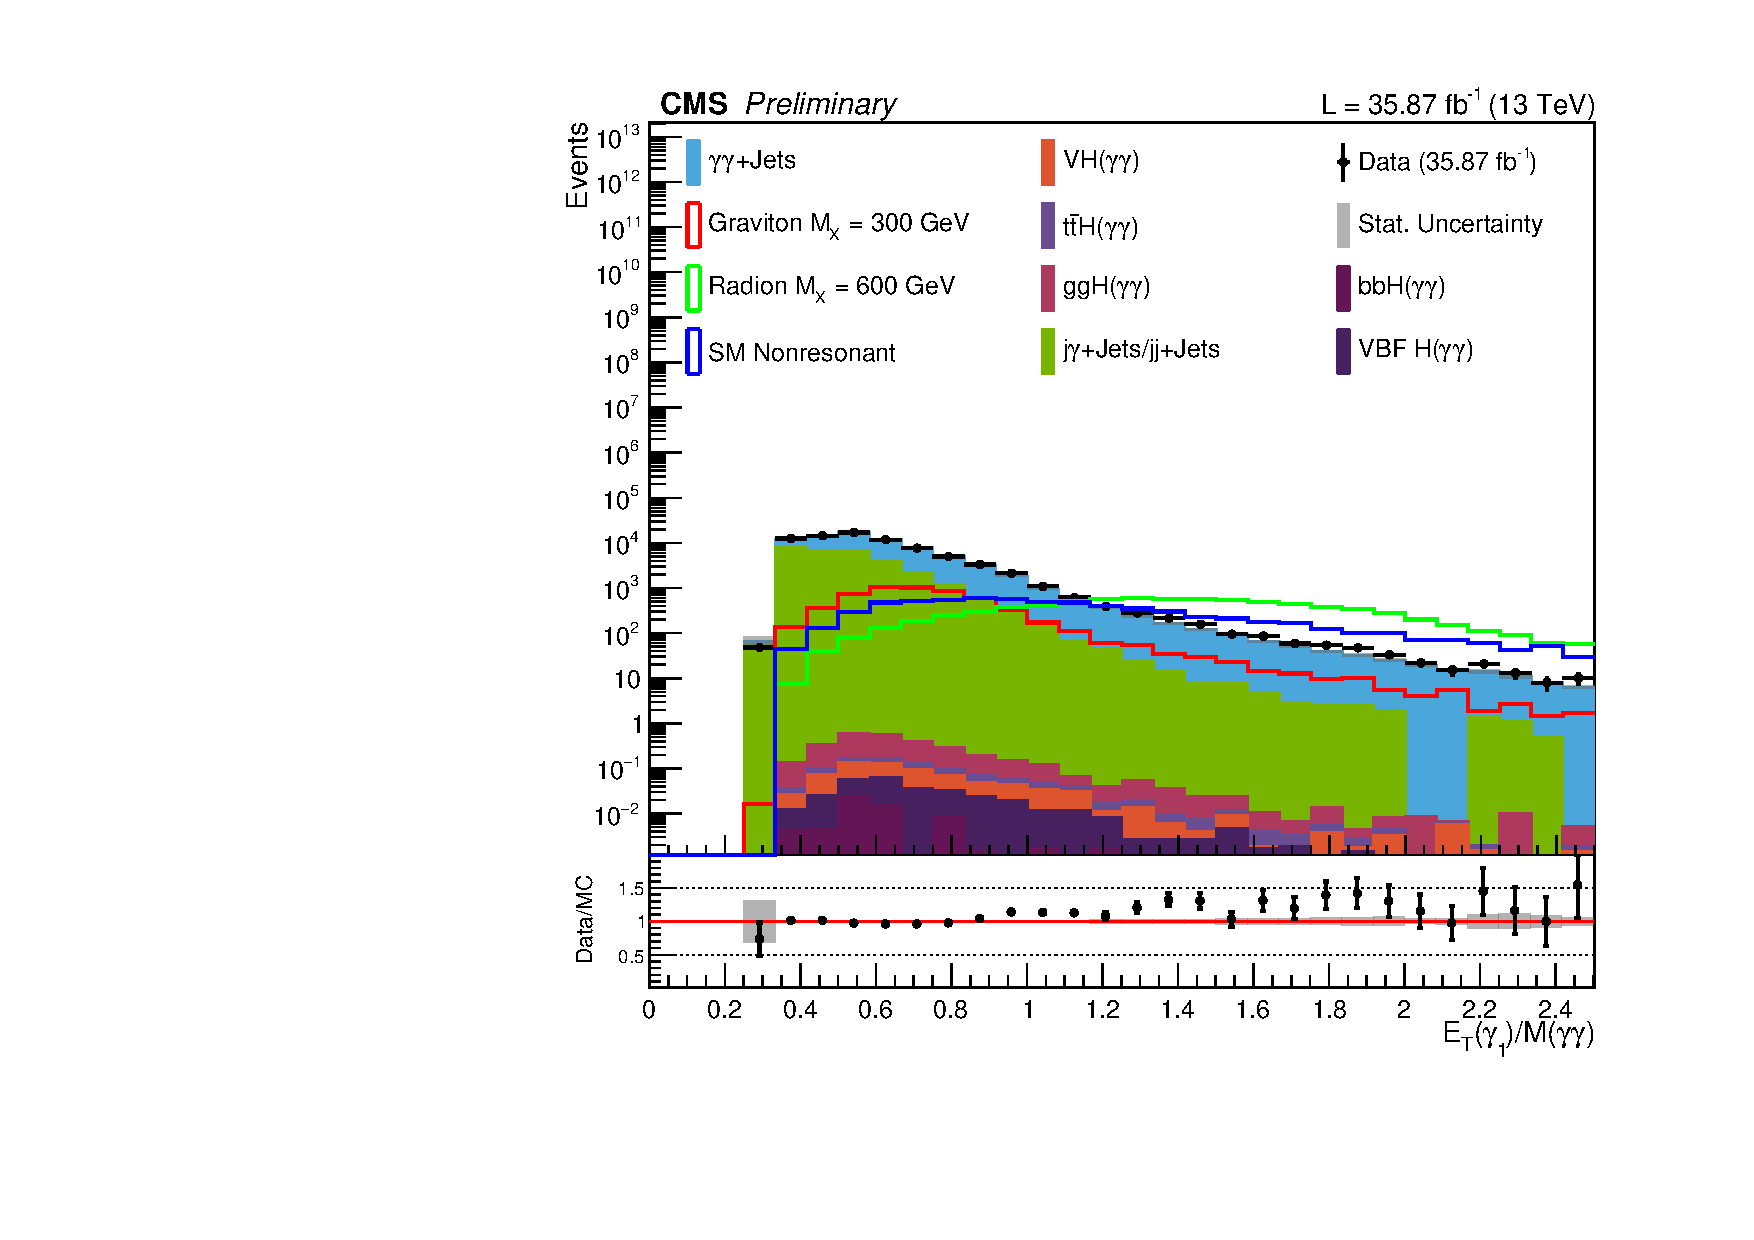
\includegraphics[width=0.45\textwidth]{figures/sec-control/LOG_lphoptmgg}\hfil

  \caption{Distributions of data and MC for the signal region with the blinding region removed. Top left: $|cos(\theta^{*}_{\gamma\gamma})|$. Top right: $p_{T}(\gamma\gamma)/M(jj\gamma\gamma)$. Center left: $p_{T}(jj)/M(jj\gamma\gamma)$. Center right: leading jet $p_{T}(j)/\Mjj$. Bottom left: subleading jet $p_{T}(j)/\Mjj$. Bottom right: leading photon $E_{T}(\gamma)/\Mjj$}
\label{fig:cp_mgg4}
\end{figure*}

%\begin{figure*}[thb]
%  \centering
%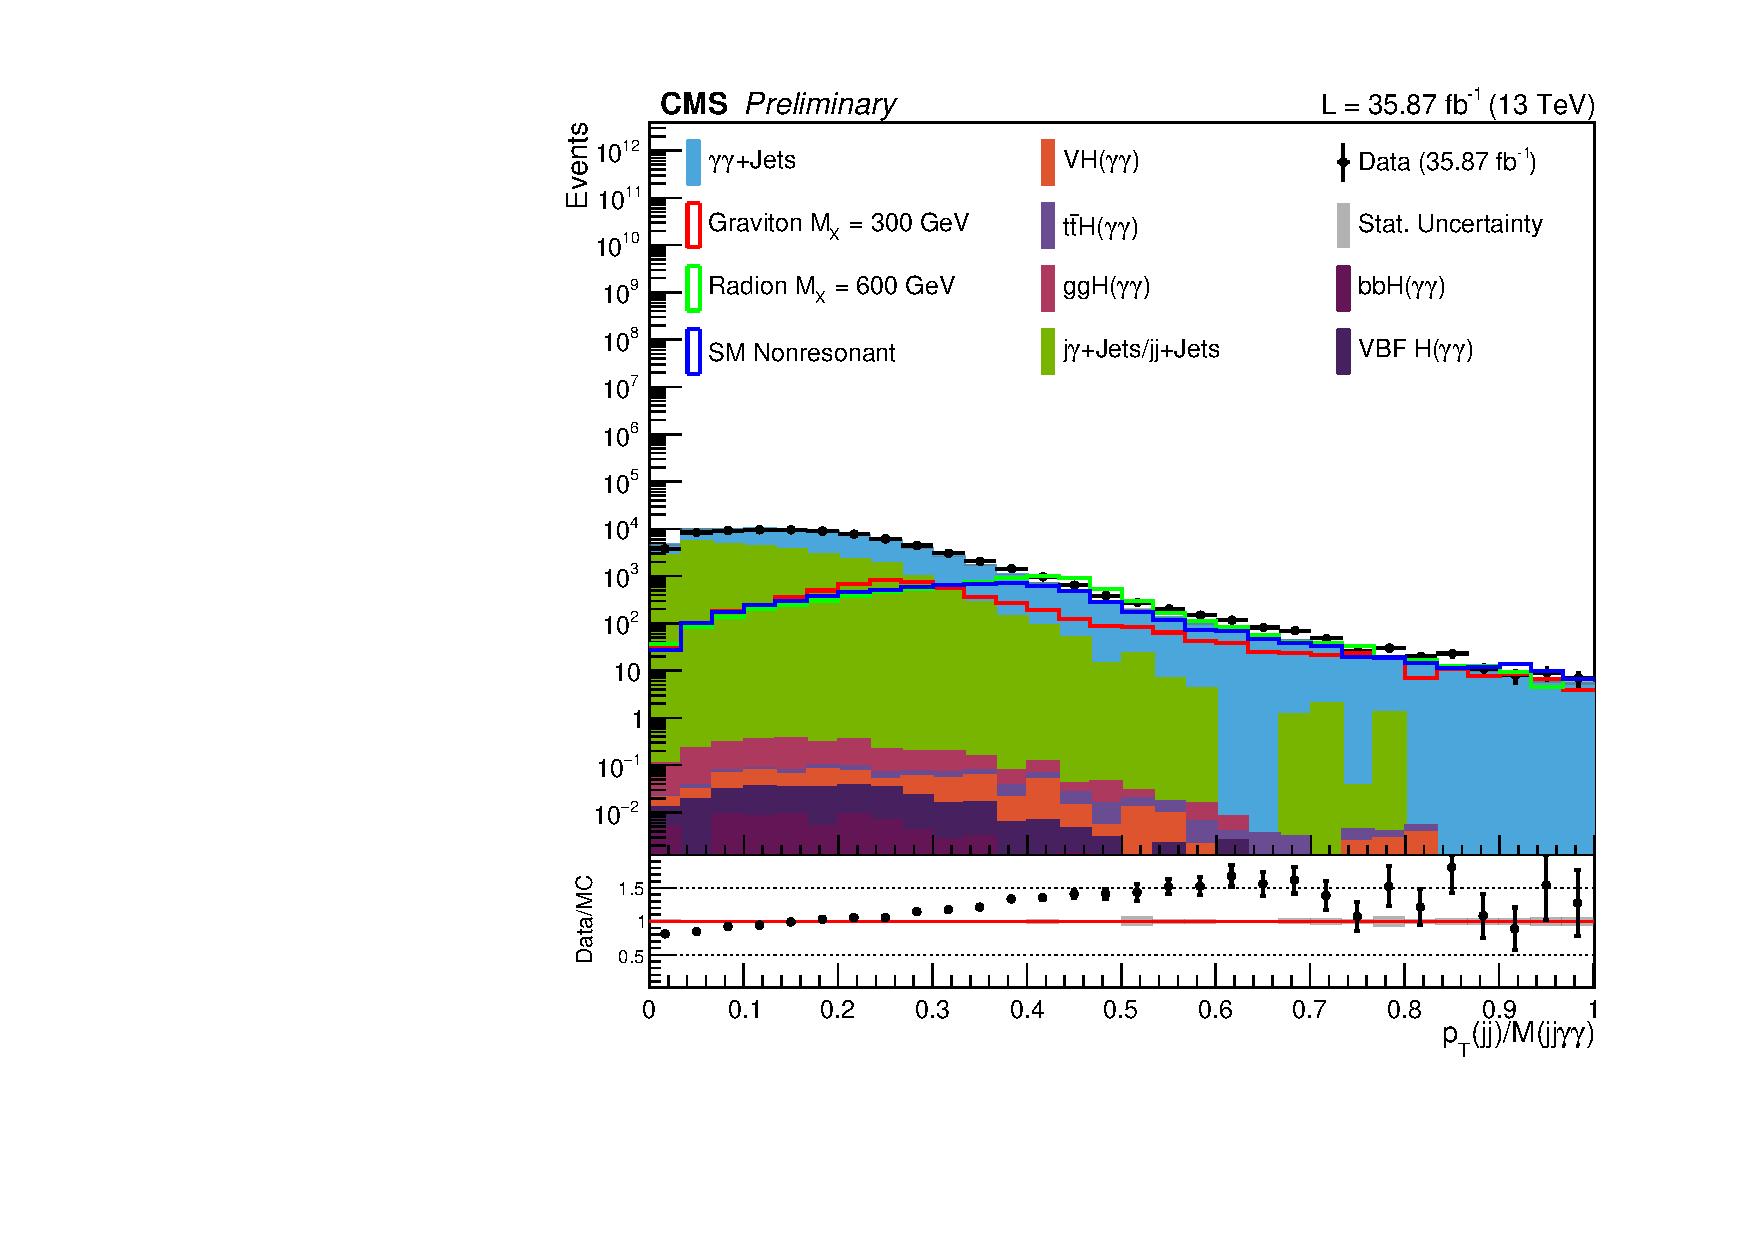
\includegraphics[width=0.45\textwidth]{figures/sec-control/LOG_jjptmjjgg.pdf}\hfil
%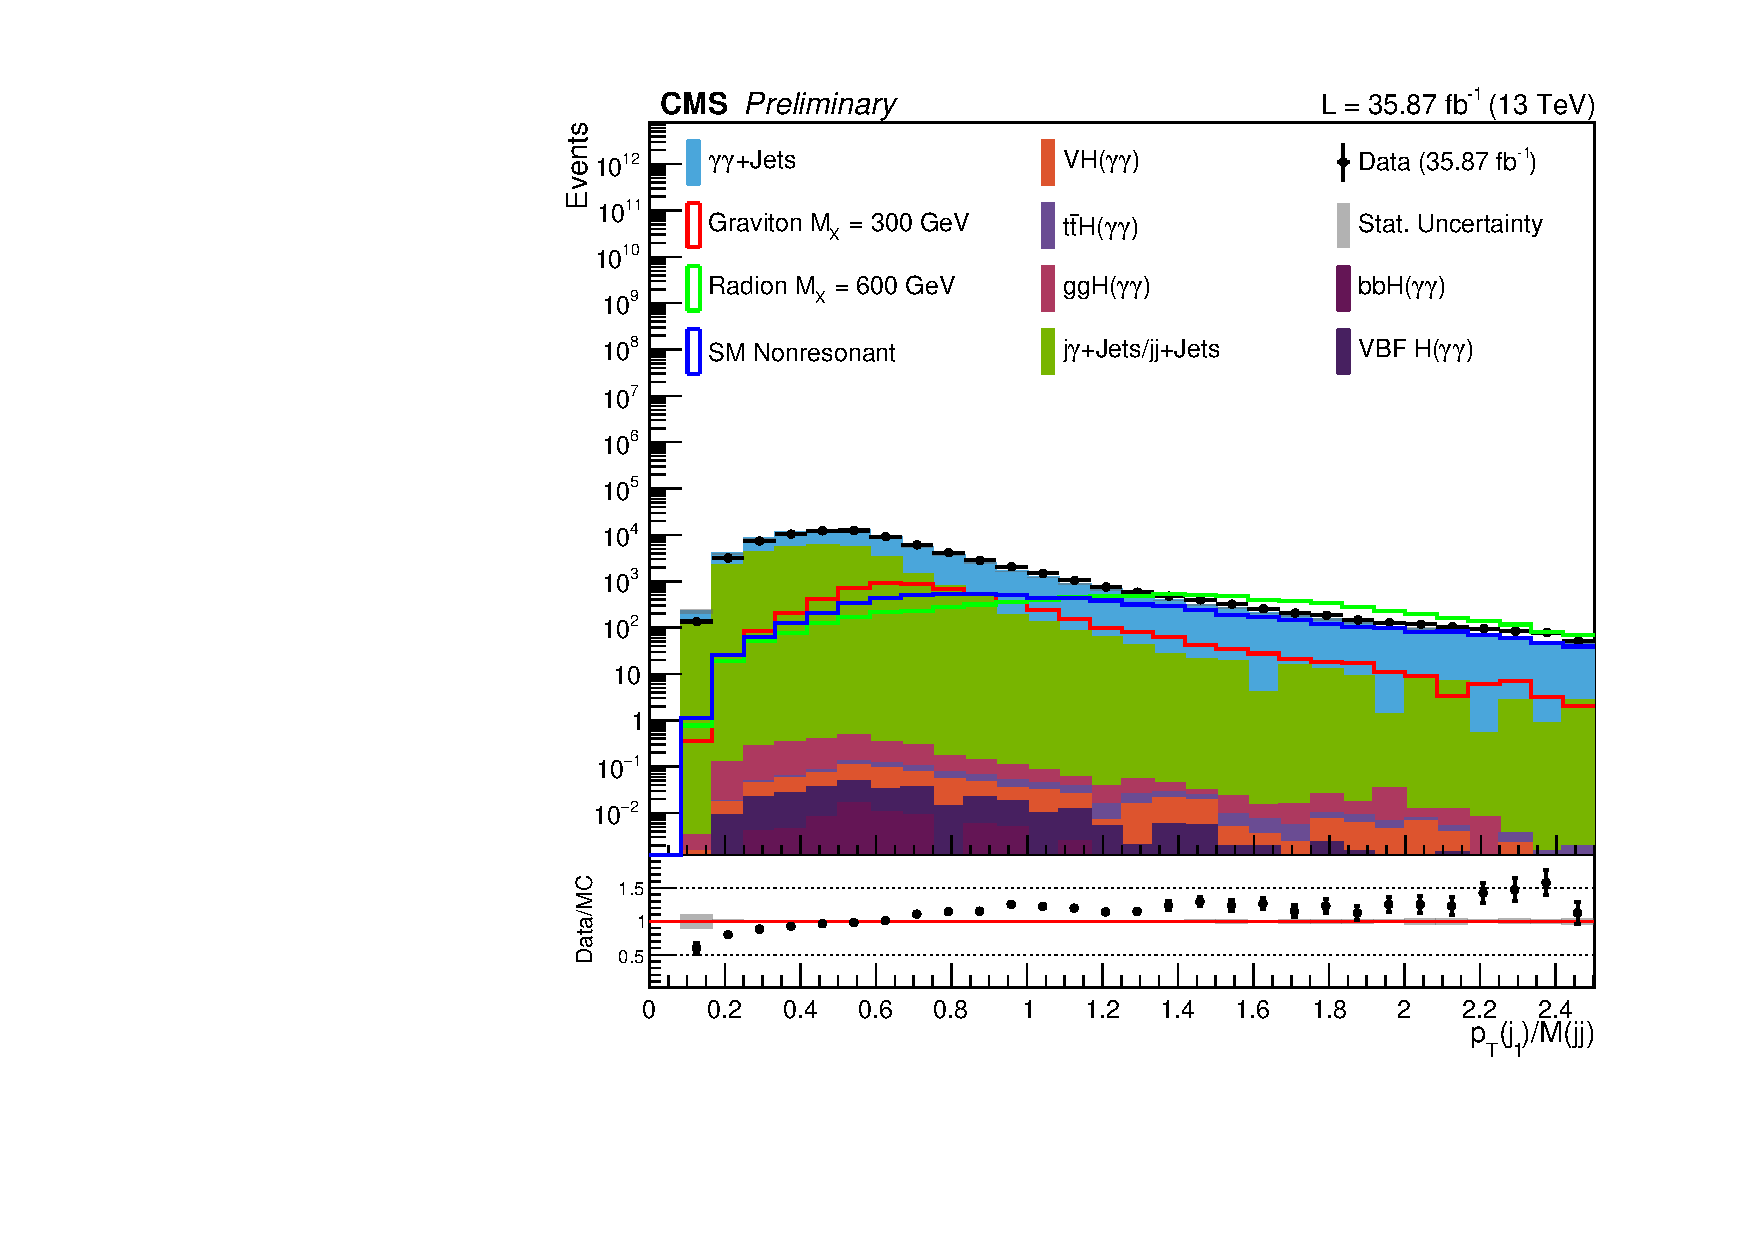
\includegraphics[width=0.45\textwidth]{figures/sec-control/LOG_ljetptmgg}\hfil
%  \caption{Distributions of data and MC for the signal region with the blinding region removed.}
%\label{fig:cp_mgg5}
%\end{figure*}
%\begin{figure*}[thb]
%  \centering
%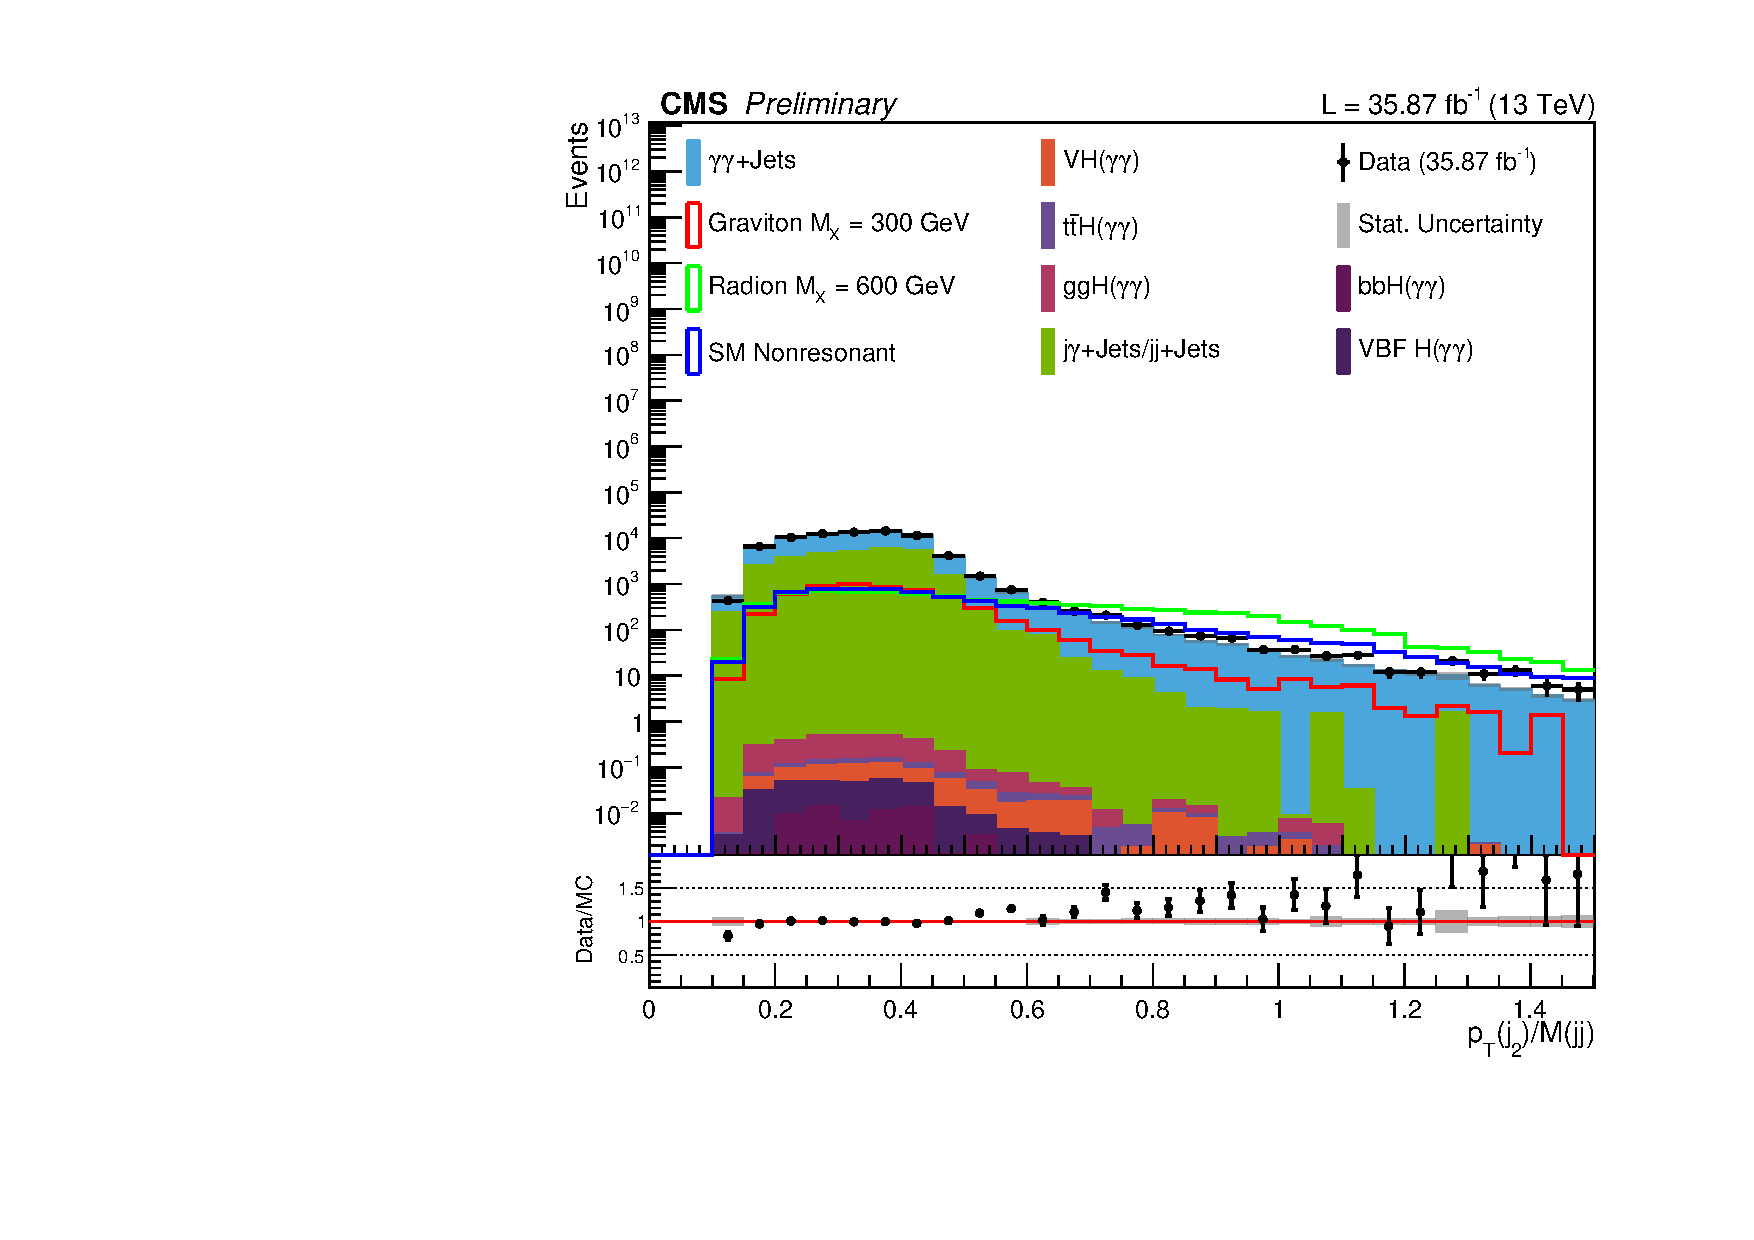
\includegraphics[width=0.45\textwidth]{figures/sec-control/LOG_sjetptmgg}\hfil
%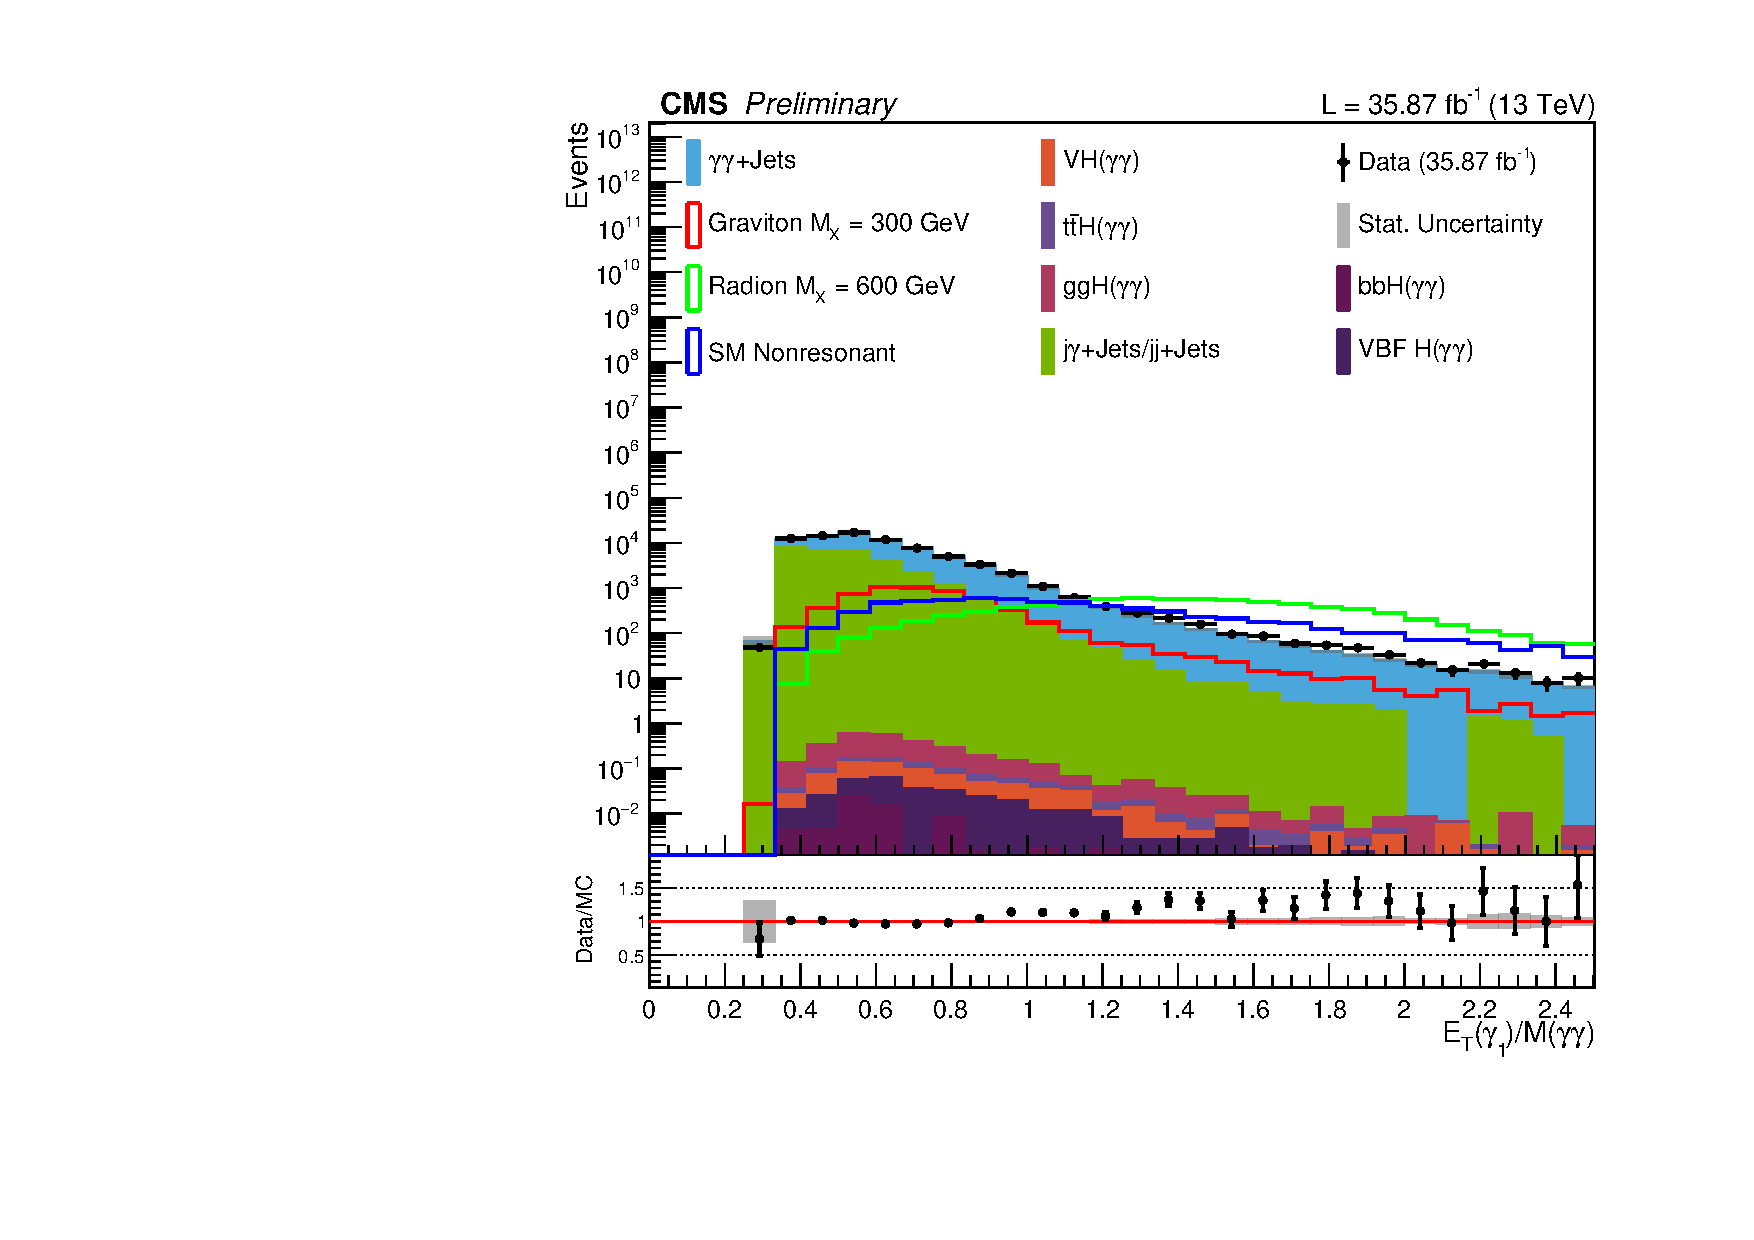
\includegraphics[width=0.45\textwidth]{figures/sec-control/LOG_lphoptmgg}\hfil
%  \caption{Distributions of data and MC for the signal region with the blinding region removed.}
%\label{fig:cp_mgg6}
%\end{figure*}

%\begin{figure*}[thb]
%  \centering
%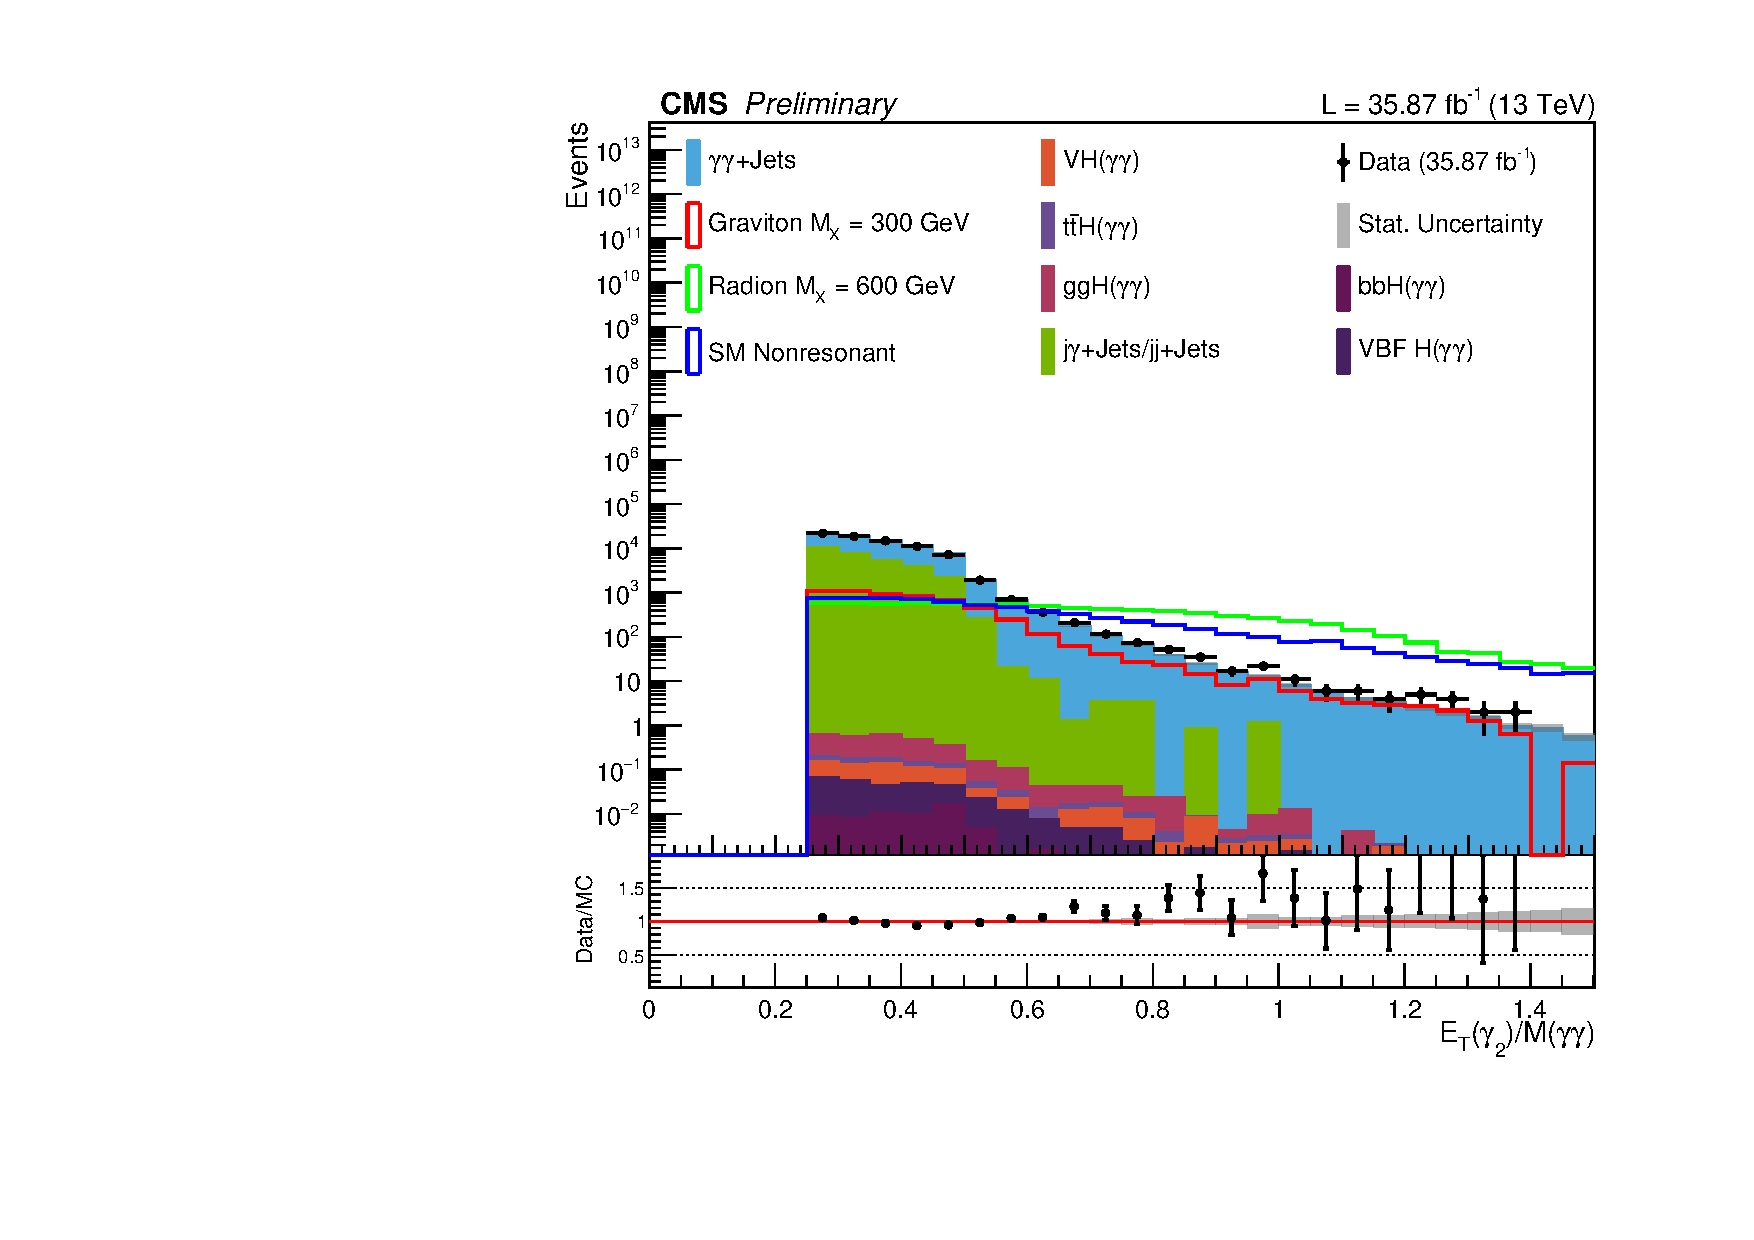
\includegraphics[width=0.45\textwidth]{figures/sec-control/LOG_sphoptmgg}\hfil
%  \caption{Distributions of data and MC for the signal region with the blinding region removed.}
%\label{fig:cp_mgg7}
%\end{figure*}
\begin{figure*}[thb]
  \centering
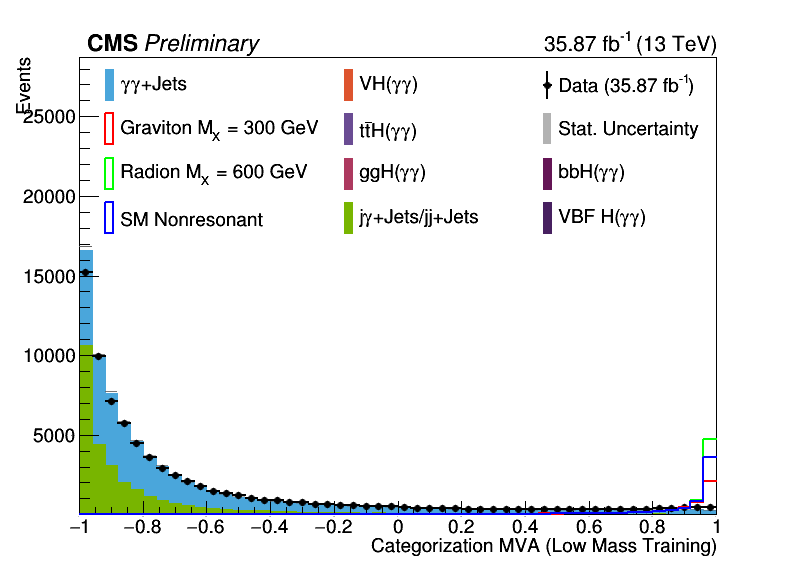
\includegraphics[width=0.65\textwidth]{figures/sec-control/NP_HHTagger_LM}
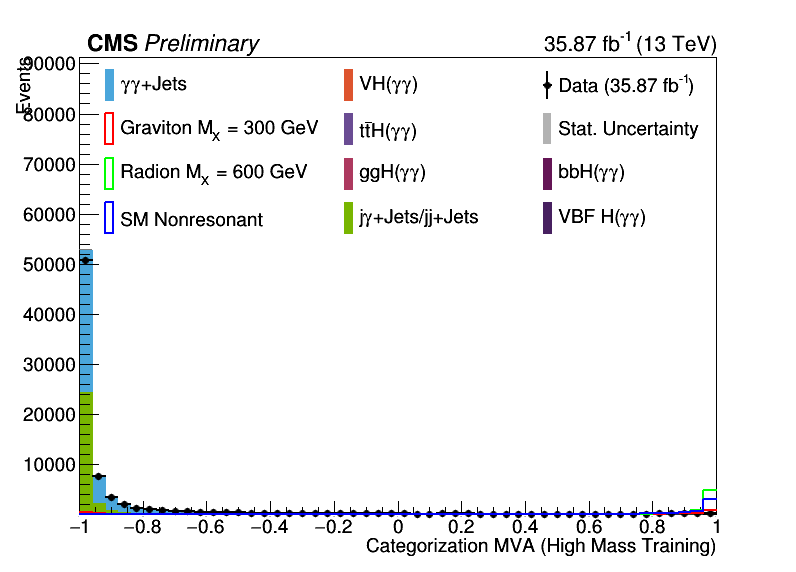
\includegraphics[width=0.65\textwidth]{figures/sec-control/NP_HHTagger_HM}
  \caption{Distributions of data and MC for the signal region with the blinding region removed. Top: Categorization MVA output (low mass training). Bottom: Categorization MVA output (high mass training).}
\label{fig:cp_mgg8}
\end{figure*}

